\documentclass[11pt]{article}
\usepackage[letterpaper,margin=1in,footskip=24pt]{geometry}
\usepackage[utf8]{inputenc}
\usepackage[T1]{fontenc}
\usepackage[english]{babel}
\usepackage{pifont}
\usepackage[numbers,super,sort,compress]{natbib}
\usepackage[colorlinks]{hyperref}
\usepackage{mathtools}
\usepackage[capitalise,noabbrev,nameinlink]{cleveref}
\usepackage[hypcap=false]{caption}
\usepackage[hang,flushmargin,symbol]{footmisc}
\usepackage{booktabs}
\usepackage{array}
\usepackage{fancyhdr}
\usepackage{xcolor}
\usepackage{xparse}
\usepackage{xpatch}
\usepackage{tabularray}
\usepackage{environ}
\usepackage{changepage}
\usepackage{lineno}
\usepackage{subcaption}
\usepackage{graphicx}
\usepackage{amsfonts}
\usepackage{nicefrac}
\usepackage{enumitem}
\usepackage{titlesec}
\usepackage{xspace}
\usepackage{wrapfig}
\usepackage[noend]{algpseudocode}
\usepackage{algorithm}

\RequirePackage{XCharter}
\RequirePackage[xcharter,bigdelims,vvarbb]{newtxmath}
\RequirePackage[scaled=1.1]{zlmtt}

\newcommand{\method}{Dreamer~4\xspace}
\newcommand{\Method}{Dreamer~4\xspace}

% Page
\setlength{\skip\footins}{24pt}

% Title page
\fancypagestyle{plain}{%
\fancyhead[L]{
\includegraphics[width=90pt]{logo}}
\fancyhead[C]{}
\fancyhead[R]{}
\fancyfoot[L]{\small%
* Equal contribution.\enskip
Google DeepMind, San Francisco, USA.\enskip
% Contact: mail@danijar.com \\[.5ex]
Website: \href{https://danijar.com/dreamer4}{danijar.com/dreamer4}
}
\fancyfoot[C]{}
\fancyfoot[R]{\small\thepage}
\renewcommand{\headrulewidth}{1pt}
\renewcommand{\footrulewidth}{1pt}
}

% Other pages
\fancypagestyle{fancy}{%
\fancyhead[L]{}
\fancyhead[C]{}
\fancyhead[R]{}
\fancyfoot[L]{}
\fancyfoot[C]{}
\fancyfoot[R]{\small\thepage}
\renewcommand{\headrulewidth}{0pt}
\renewcommand{\footrulewidth}{0pt}
}

% Fix warning
\setlength{\headheight}{17pt}
\addtolength{\topmargin}{-3pt}

% Title
\makeatletter
\renewcommand{\maketitle}{%
\thispagestyle{plain}%
\bgroup%
\begin{center}%
\vspace*{0pt}%
{\bfseries\fontsize{20pt}{20pt}\selectfont\@title\par}
\vspace*{12pt}%
{\normalsize\@author\par}
\vspace*{10pt}%
\end{center}%
\egroup}
\makeatother

% Section number periods
\titleformat{\section}{\normalfont\Large\bfseries}{\thesection.}{.5em}{}
\titleformat{\subsection}{\normalfont\large\bfseries}{\thesubsection.}{.5em}{}

% Formatting
\definecolor{linkcolor}{rgb}{0.0,0.15,0.7}
\hypersetup{colorlinks=true,allcolors=linkcolor}
\setlength\parindent{0pt}
\setlength{\parskip}{.5\baselineskip}
\bibliographystyle{unsrtnat}
\captionsetup{labelfont=bf}
\setlist[itemize]{leftmargin=1.2em,labelsep=.7em,itemsep=0ex,topsep=0ex}
\renewcommand{\paragraph}[1]{\textbf{#1}\hspace{3ex}\removeParAfter}

% Tables
\UseTblrLibrary{booktabs}
\NewTblrColumnType{L}[1]{Q[l,m,wd=#1]}
\NewTblrColumnType{C}[1]{Q[c,m,wd=#1]}
\NewTblrColumnType{R}[1]{Q[r,m,wd=#1]}
\renewcommand{\o}{\hphantom{0}}
\NewEnviron{mytabular}[1]{%
\setlength\heavyrulewidth{1.2pt}
\setlength\lightrulewidth{.5pt}
\setlength\aboverulesep{.4ex}%
\setlength\belowrulesep{.8ex}%
\begin{booktabs}[expand=\BODY]{#1}
\BODY
\end{booktabs}
}

% References
\crefname{equation}{}{}
\crefname{algocf}{Algorithm}{Algorithms}
\Crefname{algocf}{Algorithm}{Algorithms}

% Pseudocode
\makeatletter
\newcommand{\algmargin}{\the\ALG@thistlm}
\makeatother
\algrenewcommand{\alglinenumber}[1]{$\bullet$}
\algdef{SxnE}[REPEATPLAIN]{RepeatPlain}{End}[0]{\algorithmicrepeat}{}
\newcommand{\CommentClean}[1]{\Statex\hspace*{-2.5ex}\texttt{// #1}}
\algnewcommand{\ParState}[1]{\State\parbox[t]{\dimexpr\linewidth-\algmargin}{\strut#1\strut}}
\algnewcommand{\ParStateIndent}[1]{\State\quad\parbox[t]{\dimexpr\linewidth-\algmargin}{\strut#1\strut}}

% TODOs
\makeatletter
\DeclareDocumentCommand\todo{g}{%
\def\@message{\IfNoValueTF{#1}{TODO}{TODO: #1}}
\textbf{\textcolor[HTML]{FF8811}{\@message}}
\@latex@warning{\@message}{}{}}
\makeatother

% Equation
\makeatletter
\newcommand{\removeParBefore}{\ifvmode\vspace*{-\baselineskip}\setlength{\parskip}{0ex}\fi}
\newcommand{\removeParAfter}{\@ifnextchar\par\@gobble\relax}
\newcommand{\eq}{\begingroup\removeParBefore\endlinechar=32 \eqinner}
\newcommand{\eqinner}[2][aligned]{\endlinechar=32%
\begin{gather}\begin{#1}#2\end{#1}\end{gather}\endgroup\removeParAfter}
\makeatother

% Density
\DeclareDocumentCommand{\p}{ D<>{p} D<>{} r() }{%
\def\content{#3}\patchcmd{\content}{|}{\;#2\vert\;}{}{}
\ensuremath{#1 #2(\content #2)}}

% Expectation
\DeclareDocumentCommand{\E}{ D<>{E} E{_}{{}} D<>{\big} r[] }{%
\def\content{#4}\patchcmd{\content}{|}{\;#3\vert\;}
{}\ensuremath{\operatorname{#1}_{#2}#3[\content #3]}}

% Helpers
\newcommand{\tlap}[1]{\vbox to 0pt{\vss\hbox{#1}}}
\newcommand{\blap}[1]{\vbox to 0pt{\hbox{#1}\vss}}
\newcommand{\cmark}{\textcolor{green}{\ding{51}}}
\newcommand{\xmark}{\textcolor{red}{\ding{55}}}
\renewcommand{\o}{\hphantom{0}}
\newcommand{\sg}{\operatorname{sg}}
\newcommand{\EMA}{\operatorname{EMA}}
\newcommand{\dhalf}{\textstyle\frac{d}{2}}
\newcommand{\sig}{\tau}  % t, m, s, alpha
\newcommand{\dis}{d}


\title{\vspace*{-1.7ex}Training Agents Inside of Scalable World Models\vspace*{-.2ex}}

\date{}

\author{%
Danijar Hafner*\quad
Wilson Yan*\quad
Timothy Lillicrap
}

\begin{document}

\maketitle
\pagestyle{fancy}

% \linenumbers
% \begin{adjustwidth}{1cm}{1cm}
\vspace*{-2ex}
% \begin{hyphenrules}{nohyphenation}
{\ignorespaces\bfseries%
World models learn general knowledge from videos and simulate experience for training behaviors in imagination, offering a path towards intelligent agents.
However, previous world models have been unable to accurately predict object interactions in complex environments.
% Slow generation further limits their practicality for training agents.
We introduce \method, a scalable agent that learns to solve control tasks by reinforcement learning inside of a fast and accurate world model.
In the complex video game Minecraft, the world model accurately predicts object interactions and game mechanics, outperforming previous world models by a large margin.
The world model achieves real-time interactive inference on a single GPU through a shortcut forcing objective and an efficient transformer architecture.
Moreover, the world model learns general action conditioning from only a small amount of data, allowing it to extract the majority of its knowledge from diverse unlabeled videos.
We propose the challenge of obtaining diamonds in Minecraft from only offline data, aligning with practical applications such as robotics where learning from environment interaction can be unsafe and slow.
This task requires choosing sequences of over 20,000 mouse and keyboard actions from raw pixels.
By learning behaviors in imagination, \method is the first agent to obtain diamonds in Minecraft purely from offline data, without environment interaction.
Our work provides a scalable recipe for imagination training, marking a step towards intelligent agents.
}
% \end{hyphenrules}
% \end{adjustwidth}

\vfill
\vfill
\begin{figure}[t!]
\vspace*{-2\baselineskip}
\centering
\begin{subfigure}[t]{0.45\textwidth}
\centering
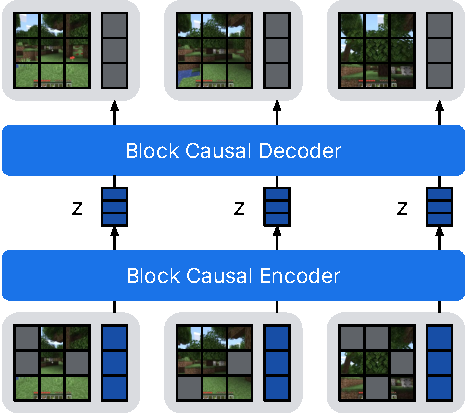
\includegraphics[height=2.4in]{figures/method/tok}
\caption{Causal Tokenizer}
\end{subfigure}%
\hfill%
\begin{subfigure}[t]{0.45\textwidth}
\centering
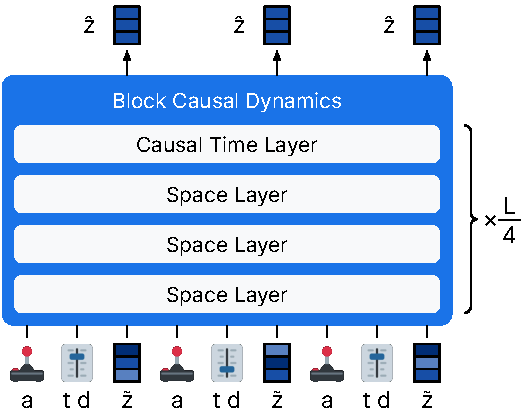
\includegraphics[height=2.5in]{figures/method/dyn}
\caption{Interactive Dynamics}
\end{subfigure}
\caption{World model design.
\method consists of a causal tokenizer and an interactive dynamics model, which both use the same block-causal transformer architecture.
The tokenizer encodes partially masked image patches and latent tokens, squeezes the latents through a low-dimensional projection with tanh activation, and decodes the patches.
It uses causal attention to achieve temporal compression while allowing frames to be decoded one by one.
The dynamics model operates on the interleaved sequence of actions, shortcut noise levels and step sizes, and tokenizer representations.
It denoises representations via a shortcut forcing objective.
After pretraining, the world model is finetuned into an agent by inserting task tokens into the dynamics transformer and predicting actions, rewards, and values from them.
}
\label{fig:model}
\end{figure}
\vfill
\clearpage

\section{Introduction}

To solve complex tasks in embodied environments, intelligent agents need to deeply understand the world and choose successful actions.
World models offer a promising approach towards this goal by learning to predict the future outcomes of potential actions from the perspective of an agent, such as a robot or a video game player.
This way, world models equip agents with a deep understanding of the world and the ability to choose actions by planning or reinforcement learning in imagination.
Moreover, world models can in principle learn from fixed datasets, allowing to train agents purely in imagination without the need for online interaction.
Optimizing behaviors offline is valuable for many practical applications, such as robots in the physical world, where online interaction with a partially trained agent is often unsafe.

World model agents, such as Dreamer~3, are among the best-performing and most robust reinforcement learning algorithms for games and robotics to date \citep{dreamerv3,wu2023daydreamer,hansen2023tdtmpc2,alonso2024diffusion,schrittwieser2019muzero,hessel2021muesli}.
While these models are fast and accurate for their narrow environments, their architecture lacks the ability to fit complex real world distributions.
Controllable video models, such as Genie~3, have been trained on diverse real video and games and have accomplished diverse scene generation and simple interactions \citep{genie3,tu2025playerone,he2025matrix,sun2025virtual,bai2025whole,team2025yan}.
These models are based on scalable architectures, such as diffusion transformers\citep{peebles2023dit,diffusionforcing}.
However, they still struggle to learn the precise physics of object interactions and game mechanics, limiting their usefulness for training successful agents.
Moreover, they often require many GPUs to simulate a single scene in real time, further reducing their practicality for imagination training.

We introduce \method, a scalable agent that solves control tasks by imagination training inside of a fast and accurate world model.
\method is the first agent to obtain diamonds in the challenging video game Minecraft purely from a standard offline dataset, without environment interaction.
\method leverages a novel shortcut forcing objective and an efficient transformer architecture to accurately learn complex object interactions while enabling real-time human interaction and efficient imagination training.
We show that the world model accurately predicts a wide range of semantic interactions in Minecraft, outperforming previous world models by a large margin.
Moreover, \method can be trained on large amounts of unlabeled videos and requires only a small amount of videos paired with actions.
This opens up the possibility of learning general world knowledge from diverse web videos in the future, for which action labels are not available.

Our contributions are summarized as follows:

\begin{itemize}
\item We introduce \method, a scalable agent that learns to solve challenging control tasks by imagination training inside of a world model.
\item \method is the first agent to collect diamonds in Minecraft from only offline data, substantially improving over OpenAI's VPT offline agent\citep{vpt} despite using 100$\times$ less data.
\item We introduce a high-capacity world model that achieves real-time inference on a single GPU through a shortcut forcing objective and an efficient transformer architecture.
\item We show that the world model accurately predicts a wide range of object interactions and game mechanics in Minecraft, substantially outperforming previous world models.
\item We show that the world model can learn from unlabeled videos and requires only a small amount of aligned data to learn action conditioning with strong generalization.
\item An extensive ablation study measures the improvements of the objective and architecture.
\end{itemize}

\section{Background}
\label{sec:background}

\paragraph{Flow matching}

Our world model is based on the paradigm of diffusion models~\citep{sohl2015deep,ddpm}, where the network $f_\theta$ is trained to restore the a data point $x_1$ given a corrupted version $x_\sig$.
The signal level $\sig \in [0, 1]$ determines the mixture of noise and data and is randomized during training, where $\sig=0$ corresponds to pure noise and $\sig=1$ means clean data.
We build on the flow matching formulation~\citep{flowmatching,rectifiedflow} because of its simplicity, where the network predicts the velocity vector $v = x_1 - x_0$ that points towards the clean data:

\eq{
\begin{gathered}
x_\sig = (1 - \sig)\,x_0 + \sig\,x_1 \qquad
x_0 \sim \operatorname{N}(0, \mathbb{I}) \qquad
x_1 \sim \mathcal{D} \qquad
\sig \sim \p(\sig) \\[1.5ex]
\mathcal{L}(\theta) = \| f_\theta(x_\sig,\sig) - (x_1 - x_0) \|^2
\end{gathered}
}

The signal level is typically sampled from a uniform distribution or a logit-normal distribution \citep{sd3}.
At inference time, the sampling process starts with a pure noise vector $x_0$ and iteratively transforms it into a clean data point $x_1$ over $K$ sampling steps with step size $d = 1/K$:

\eq{
x_{\sig+\dis} = x_\sig + f_\theta(x_\sig,\sig)\,\dis \qquad
x_0 \sim \operatorname{N}(0, \mathbb{I})
}

\paragraph{Shortcut models}

Shortcut models \citep{shortcut} condition the neural network not only on the signal level $\sig$ but also on the requested step size $\dis$.
This allows them to choose the step size at inference time and generate data points using only a few sampling steps and forward passes of the neural network.
For the finest step size $\dis_\mathrm{min}$, shortcut models are trained using the flow matching loss.
For larger step sizes $\dis_\mathrm{min}<\dis \leq 1$, shortcut models are trained using a bootstrap loss that distills two smaller steps, where $\operatorname{sg}(\cdot)$ stops the gradient:

\eq{
\begin{gathered}

x_0 \sim \operatorname{N}(0, \mathbf{I}) \qquad
x_1 \sim \mathcal{D} \qquad
\sig,\dis \sim \p(\sig,\dis) \\[1.2ex]

b' = f_\theta(x_\sig,\sig,\dis/2) \qquad
b'' = f_\theta(x',\sig+\dis/2,\dis/2) \qquad
x' = x_\sig + b'\,\dis/2 \\

\mathcal{L}(\theta) = \| f_\theta(x_\sig,\sig,\dis) - v_\mathrm{target} \|^2
\qquad
v_\mathrm{target} = \begin{cases}
x_1 - x_0 &\text{if } \dis=\dis_\mathrm{min}  \\
\sg(b' + b'')/2 &\text{else}
\end{cases}

\end{gathered}
}

The step size is sampled uniformly as a power of two, based on the maximum number of sampling steps $K_\mathrm{max}$, which defines the finest step size $\dis_\mathrm{min}=1/K_\mathrm{max}$. The signal level is sampled uniformly over the grid that is reached by the current step size:

\eq{
\dis \sim 1/\operatorname{U}(\{1, 2, 4, 8, \dots, K_{\mathrm{max}}\}) \qquad
\sig \sim \operatorname{U}(\{0, 1/\dis, \dots, 1 - 1/\dis\})
}

At inference time, one can condition the model on a step size $\dis=1/K$ to target $K$ sampling steps, without suffering from discretization error because the model has learned to predict the end point of each step. In practice, shortcut models generate high-quality samples with 2 or 4 sampling steps, compared to 64 or more steps for typical diffusion models.

\paragraph{Diffusion forcing}

For sequential data, diffusion forcing \citep{diffusionforcing} assigns a different signal level to each time step of the data sequence, producing a corrupted sequence.
This allows applying loss terms to all time steps in the sequence, where each time step serves both as denoising task and as history context for later time steps.
At inference time, diffusion forcing supports flexible noise patterns, such as generating the next frame given clean or lightly noised history.

\pagebreak
\section{World Model Agent}

\begin{wrapfigure}[21]{R}{0.44\textwidth}
\vspace*{-5ex}\hfill%
\begin{minipage}{0.43\textwidth}
\begin{algorithm}[H]
\caption{\enskip\method}
\label{alg:agent}
\begin{hyphenrules}{nohyphenation}

\begin{algorithmic}[1]
\setlength{\itemsep}{.5ex}

\vspace{1ex}
\Statex \hspace*{-2.3ex}\textbf{Phase 1:} World Model Pretraining
\State Train tokenizer on videos using \cref{eq:tok}.
\State Train world model on tokenized videos and optionally actions using \cref{eq:dyn}.

\vspace{1ex}
\Statex \hspace*{-2.3ex}\textbf{Phase 2:} Agent Finetuning
\State Finetune world model with task inputs for policy and reward heads using \cref{eq:dyn} and \cref{eq:bcrm}.

\vspace{1ex}
\Statex \hspace*{-2.3ex}\textbf{Phase 3:} Imagination Training
\State Optimize policy head using \cref{eq:pol} and value head using \cref{eq:val} on trajectories generated by the world model and the policy head.
\vspace{1ex}

\end{algorithmic}
\end{hyphenrules}
\end{algorithm}
\end{minipage}
\end{wrapfigure}
We present \method, a scalable agent that learns to solve complex control tasks by reinforcement learning inside of a fast and accurate world model.
The agent consists of a tokenizer and a dynamics model, as shown in \cref{fig:model}.
The tokenizer compresses video frames into continuous representations and the dynamics model predicts the representations given interleaved actions, both using the same efficient transformer architecture.
The tokenizer is trained using masked autoencoding and the dynamics is trained using a shortcut forcing objective to enable interactive generations with a small number of forward passes and prevent accumulating errors over time.
As outlined in \cref{alg:agent}, we first pretrain the tokenizer and world model on videos and actions, then finetune the policy and reward model into the world model by interleaving task embeddings, and finally post-train the policy through imagination training.
To train a single dynamics transformer with multiple modalities and output heads, we normalize all loss terms by running estimates of their root-mean-square (RMS).

\begin{figure}[t!]
\vspace*{-2\baselineskip}
\centering
\begin{subfigure}[t]{0.45\textwidth}
\centering
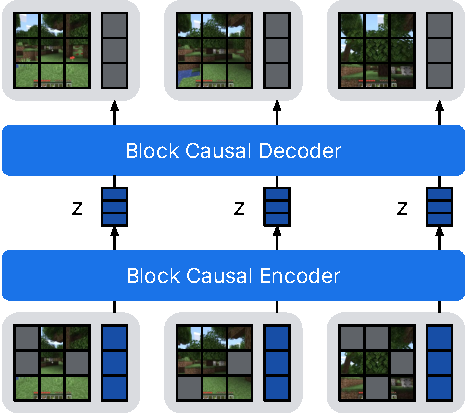
\includegraphics[height=2.4in]{figures/method/tok}
\caption{Causal Tokenizer}
\end{subfigure}%
\hfill%
\begin{subfigure}[t]{0.45\textwidth}
\centering
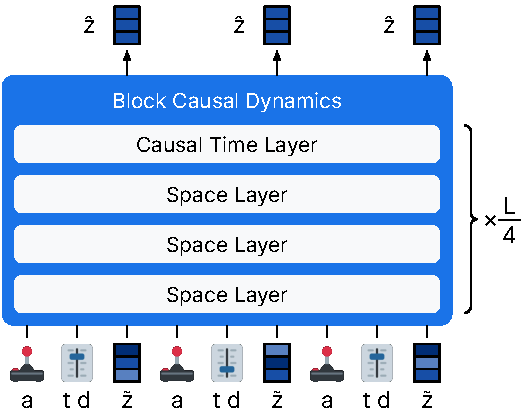
\includegraphics[height=2.5in]{figures/method/dyn}
\caption{Interactive Dynamics}
\end{subfigure}
\caption{World model design.
\method consists of a causal tokenizer and an interactive dynamics model, which both use the same block-causal transformer architecture.
The tokenizer encodes partially masked image patches and latent tokens, squeezes the latents through a low-dimensional projection with tanh activation, and decodes the patches.
It uses causal attention to achieve temporal compression while allowing frames to be decoded one by one.
The dynamics model operates on the interleaved sequence of actions, shortcut noise levels and step sizes, and tokenizer representations.
It denoises representations via a shortcut forcing objective.
After pretraining, the world model is finetuned into an agent by inserting task tokens into the dynamics transformer and predicting actions, rewards, and values from them.
}
\label{fig:model}
\end{figure}

\pagebreak
\subsection{Causal Tokenizer}
\label{sec:tokenizer}

The tokenizer compresses raw video into a sequence of continuous representations for the dynamics model to consume and generate.
It consists of an encoder and a decoder with a bottleneck in between.
Both components are causal in time, enabling temporal compression while maintaining the ability to decode frame by frame for interactive inference.

\paragraph{Architecture}

We use the efficient transformer architecture described later.
Each time step consists of patch tokens of the current image and learned latent tokens.
After applying the encoder, the representations are read out of the latent tokens using a linear projection to a smaller channel dimension followed by a \texttt{tanh} activation.
For the decoder, this representation is projected back up to the model dimension and concatenated with learned tokens to read out the patches.
To flexibly integrate multiple input modalities if available, the encoder allows the latent tokens to attend to all modalities, while each modality only attends within itself.
Correspondingly, each decoder modality attends within itself and to the latents, while the latents only attend within themselves.

\paragraph{Masked autoencoding}

We train the tokenizer using a straightforward reconstruction objective, consisting of mean squared error and LPIPS \citep{lpips} loss.
To simplify weighing the two loss terms, we employ loss normalization as explained later.

\eq{
\mathcal{L}(\theta) =
\mathcal{L}_{\mathrm{MSE}}(\theta) +
0.2\,\mathcal{L}_{\mathrm{LPIPS}}(\theta)
\label{eq:tok}
}

We drop out input patches to the encoder to improve its representations using masked autoencoding \citep{mae,chen2025maetok}.
The dropout probability is randomized across images as $p \sim U(0, 0.9)$. Patches of each image are replaced with a learned embedding with this probability, so that the tokenizer is sometimes trained on the $p=0$ case used during inference.
We found MAE training to improve the spatial consistency of videos generated by the dynamics model.

\subsection{Interactive Dynamics}
\label{sec:dynamics}

The dynamics model operates on the interleaved sequence of actions and representations produced by the frozen tokenizer.
It is trained using a shortcut forcing objective to enable fast interactive inference with $K=4$ forward passes per generated frame.

\paragraph{Architecture}

The dynamics model uses our efficient transformer architecture on interleaved blocks of observations and actions.
The representations are linearly projected into $S_\mathrm{z}$ spatial tokens and concatenated with $S_\mathrm{r}$ learned register tokens \citep{vitregister} and a single token for the shortcut signal level and step size.
Since the signal level and step size are discrete, we encode each with a discrete embedding lookup and concatenate their channels.
Actions can contain multiple components, such as mouse and keyboard.
We encode each action component separately into $S_\mathrm{a}$ tokens and sum the results together with a learned embedding.
Continuous actions components are linearly projected and categorical or binary components use an embedding lookup.
When training unlabeled videos, only the learned embedding is used.

\paragraph{Shortcut forcing}

For efficient training and inference, we train the dynamics model using a shortcut forcing objective, which builds on diffusion forcing \citep{diffusionforcing} and shortcut models \citep{shortcut}, reviewed in \cref{sec:background}.
We formulate the objective in data space to prevent accumulating errors caused by high-frequency network outputs and introduce a simple loss weight to focus the model capacity on the loss terms with the most learning signal.
The dynamics model takes the interleaved sequence of actions $a=\{a_t\}$, discrete signal levels $\sig=\{\sig_t\}$ and step sizes $\dis=\{\dis_t\}$, and corrupted representations $\tilde{z}=\{z_t^{(\tau_t)}\}$ as input and predicts the clean representations $z_1=\{z_t^1\}$.
Note that $t \in [1,T]$ is the sequence timestep while $\tau_t \in [0, 1]$ is the signal level at that step.

\eq{
\begin{gathered}
z_0 \sim \operatorname{N}(0, \mathbf{1}) \qquad
z_1 \sim \mathcal{D} \qquad
\sig, \dis \sim \p(\sig, \dis) \qquad
\sig, \dis \in [0, 1]^T \\[1ex]
\hat{z}_1 = f_\theta(\tilde{z},\sig,\dis,a) \qquad
\tilde{z} = (1-\sig)\,z_0 + \sig\,z_1
\end{gathered}
}

Shortcut models parameterize the network to predict velocities $v = x_1 - x_0$, called v-prediction \citep{kingma2023understanding}.
This approach excels when generating the output jointly as one block, such as for image or video generation models.
However, v-prediction trains the network to produce high-frequency outputs.
When iteratively generating long videos frame by frame, this can cause subtle errors that accumulate over time.
Instead, we found that parameterizing the network to predict clean representations, called x-prediction, enables high-quality rollouts of arbitrary length.
Computing the flow loss term in x-space is straightforward \citep{kingma2023understanding}. To compute the bootstrap loss term, we convert the network output into v-space and scale the resulting loss back into x-space\footnote{
The network output is converted as $\hat{v}_\sig = (\hat{x}_1 - x_\sig) / (1 - \sig)$. The MSE in x-space and v-space is related by $\|\hat{x}_1 - x_1\|^2_2 = (1-\sig)^2\|\hat{v}_\sig-v_\sig\|^2_2$, motivating a $(1-\sig)^2$ multiplier to bring the bootstrap loss into a range similar to the x-space flow loss.}:

\eq{
\begin{gathered}
\begin{aligned}
b' &= (f_\theta(\tilde{z},\sig,\dhalf,a) - z_\sig)/(1-\sig) \qquad
z' = \tilde{z} + b'\,\dhalf \\
b'' &= (f_\theta(z',\sig+\dhalf,\dhalf,a) - z')/(1-(\sig+\dhalf))
\end{aligned} \\
\mathcal{L}(\theta) = \begin{cases}
\|\hat{z}_1 - z_1\|_2^2 &\text{if } \dis=\dis_\mathrm{min} \\
(1-\sig)^2 \| (\hat{z}_1-\tilde{z})/(1-\sig) - \sg(b_1 + b_2)/2  \|_2^2 &\text{else} \\
\end{cases}
\end{gathered}
\label{eq:dyn}
}

Low signal levels contain less learning signal, because the flow matching term degenerates to predicting the dataset mean, while the bootstrap term is generally easier to optimize because it has deterministic targets compared to the noisy flow matching term.
To focus the model capacity on signal levels with the most learning signal, we propose a \texttt{ramp} loss weight that linearly increases with the signal level $\sig$, where $\sig=0$ corresponds to full noise and $\sig=1$ to clean data:

\eq{
w(\sig) = 0.9 \sig + 0.1
}

At inference time, the dynamics model supports different noise patterns.
We sample autoregressively in time and generate the representations of each frame using the shortcut model with $K=4$ sample steps with corresponding step size $\dis=1/4$.
We slightly corrupt the past inputs to the dynamics model to signal level $\sig_\mathrm{ctx}=0.1$ to make the model robust to small imperfections in its generations.

\subsection{Imagination Training}

To solve control tasks, we first adapt the pretrained world model to predict actions and rewards from the dataset conditioned on one of multiple tasks.
For this, we insert agent tokens as an additional modality into the world model transformer and interleave it with the image representations, actions, and register tokens.
The agent tokens receive task embeddings as input and we use them to predict the policy and reward model using MLP heads.
While the agent tokens attend to themselves and all other modalities, no other modalities can attend back to the agent tokens.
This is crucial for avoiding causal confusion of the world model---its future predictions can only be directly influenced by actions, not by the current task.
To improve beyond strategies displayed in the dataset, we then finetune the policy through imagination training by reinforcement learning on rollouts generated by the world model, using an additional value head.

\paragraph{Behavior cloning and reward model}

After pretraining the world model on action-conditioned video prediction, the second training phase involves learning a task-conditioned policy and reward model.
Given a dataset of videos $x=\{x_t\}$ that are encoded into representations $z=\{z_t\}$, actions $a=\{a_t\}$, tasks $q=\{q_t\}$, and scalar rewards $r=\{r_t\}$, we train the policy and reward heads on the task output embeddings $h_t$ using multi-token prediction (MTP) \citep{gloeckle2024mtp} of length $L=8$:

\eq{
\mathcal{L}(\theta) =
- \sum_{n=0}^{L} \p<\ln p_\theta>(a_{t+n} | h_t)
- \sum_{n=0}^{L} \p<\ln p_\theta>(r_{t+n} | h_t)
\label{eq:bcrm}
}

To preserve existing capabilities, we reuse the pretraining setting with this additional loss function, so the representations are noisy and we continue to apply the video prediction loss.
We parameterize the policy and reward heads using small MLPs with one output layer per MTP distance.
Following Dreamer~3, the reward head is parameterized as a symexp twohot output \citep{dreamerv3} to robustly learn stochastic rewards across varying orders of magnitude.
The policy head is parameterized as categorical or vectorized binary distribution, depending on the action space of the dataset.

\paragraph{Reinforcement learning}

To improve the policy beyond behaviors displayed in the dataset, we continue training it with reinforcement learning on imagined rollouts to maximize the learned reward model.
Unlike online reinforcement learning that requires interaction with the environment, our policy learns purely inside the world model, enabling it to improve offline.
We initialize a value head and a frozen copy of the policy head that serves as a behavioral prior.
We only update the policy and value heads and keep the transformer frozen.\footnote{Finetuning the full transformer provides small additional benefits at higher computational cost. For that, the dynamics, policy prior, and reward losses need to be applied during imagination training to preserve their functions.}
%
Imagined rollouts start from contexts of the dataset that was used during the earlier training phases.
Unlike previous generations of Dreamer, we start only one rollout from each context, prioritizing data diversity and reducing memory consumption.
The rollouts are generated by unrolling the transformer with itself, sampling representations $z=\{z_t\}$ from the flow head and actions $a=\{a_t\}$ from the policy head.
We annotate the resulting trajectories with rewards $r=\{r_t\}$ using the reward head and values $v=\{v_t\}$ using the value head.

The value head is trained to predict the discounted sum of future rewards, allowing the policy to maximize rewards beyond the imagination horizon.
It uses a symexp twohot output to robustly learn across different scales of values\citep{dreamerv3}.
We train the value head using temporal difference learning (TD-learning) \citep{sutton1988td} to predict $\lambda$-returns computed from the predicted rewards and values along the sequence, where $\gamma=0.997$ is a discount factor and $c_t$ indicates non-terminal states:

\eq{
\mathcal{L}(\theta) = -\sum_{t=1}^T \ln\p<p_\theta>(R^\lambda_t | s_t)
\qquad
R^\lambda_t = r_t + \gamma c_t \big((1-\lambda)v_t + \lambda R^\lambda_{t+1}\big)
\qquad
R^\lambda_T = v_T
\label{eq:val}
}

Unlike previous generations of Dreamer, the policy head learns using PMPO \citep{abdolmaleki2024pmpo}, a robust reinforcement learning objective that uses the sign of the advantages $A_t = R^\lambda_t-v_t$ and ignores their magnitude.
This property alleviates the need for normalizing returns or advantages and ensures equal focus on all tasks despite potentially differing return scales.
PMPO balances the focus on positive and negative feedback by separately averaging a simple maximum likelihood loss over the states with positive and negative advantages, respectively.
We assign all imagined states $s_i$ across batch and time dimensions to the positive set $\mathcal{D}^+=\{s_i \mid A_t \geq 0\}$ or the negative set $\mathcal{D}^-=\{s_i \mid A_t < 0\}$ and apply the following policy loss:

\eq{
\mathcal{L}(\theta) &=
\frac{1-\alpha}{|\mathcal{D}^-|} \sum_{i \in \mathcal{D}^-}  \ln \p<\pi_\theta>(a_i|s_i)
-\frac{\alpha}{|\mathcal{D}^+|} \sum_{i \in \mathcal{D}^+} \ln \p<\pi_\theta>(a_i|s_i)
+\frac{\beta}{N} \sum_{i=1}^N \operatorname{KL}[\p<\pi_\theta>(a_i|s_i)\,\|\,\pi_\mathrm{prior}] \\
\label{eq:pol}
}

We set $\alpha=0.5$ to balance the positive and negative sets equally and use a weaker scale of $\beta=0.3$ for the behavioral prior.
Unlike the original PMPO objective, we use a reverse direction for the prior KL to better constrain the policy to the space of reasonable behaviors.
We find the scaling between the three objective terms to be highly robust in practice as they are all measured in nats\citep{shannon1948infotheory}.

\subsection{Efficient Transformer}

Scaling up world models to diverse data distributions while maintaining fast inference requires an efficient high capacity architecture.
In this section, we introduce our efficient transformer architecture that is used for both the tokenizer and the dynamics model.
The architecture is a 2D transformer \citep{vaswani2017transformer} with time and space dimensions.
To support interactive generation, the attention is masked to be causal in time, so that all tokens within a time step can attend to each other and to the past.
We start from a standard transformer with pre-layer RMSNorm \citep{rmsnorm}, RoPE \citep{rope}, and SwiGLU \citep{swiglu}.
We employ QKNorm \citep{dehghani2023scaling} and attention logit soft capping \citep{bello2016neural,gemma2} to increase training stability.

\paragraph{Efficiency}

Inference speed of block-causal transformer architectures is limited both by the FLOPs of the MLPs and the memory bandwidth needed to access the KV cache of a long context to attend into.
We employ a sequence of improvements to speed up inference, some of which also accelerate training.
First, we break up the cost of dense attention over all video tokens by using separate space-only and time-only attention layers \citep{axial}.
Second, we find that only a relatively small number of temporal layers are needed and only use temporal attention once every 4 layers, in line with recent findings \citep{llama4}.
Third, we apply GQA \citep{gqa} to all attention layers in the dynamics, where multiple query heads attend to the same key-value heads to reduce the KV cache size further.

\paragraph{Sequence length}

Increasing spatial tokens directly improves visual quality, whereas increasing temporal tokens allows training longer context lengths for more temporally consistent generation.
To support efficient training, we alternate training on many short batches and occasional long batches, and finetune the model on only long batches afterwards.
Alternating batch lengths produces intermediate training metrics and generations that are more indicative of final model performance than training only on short batches.
The batch lengths need to be longer than the context length of the model to prevent the transformer from overfitting to always seeing a start frame at the beginning of its context, enabling length generalization to arbitrary generation lengths.

\pagebreak
\section{Experiments}

\begin{figure}[t!]
\vspace*{-2\baselineskip}
\centering
\begin{subfigure}[t]{0.45\textwidth}
\centering
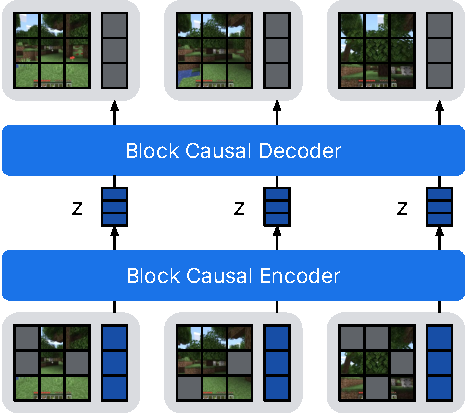
\includegraphics[height=2.4in]{figures/method/tok}
\caption{Causal Tokenizer}
\end{subfigure}%
\hfill%
\begin{subfigure}[t]{0.45\textwidth}
\centering
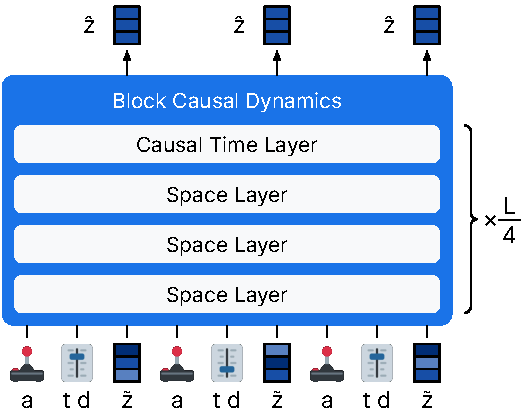
\includegraphics[height=2.5in]{figures/method/dyn}
\caption{Interactive Dynamics}
\end{subfigure}
\caption{World model design.
\method consists of a causal tokenizer and an interactive dynamics model, which both use the same block-causal transformer architecture.
The tokenizer encodes partially masked image patches and latent tokens, squeezes the latents through a low-dimensional projection with tanh activation, and decodes the patches.
It uses causal attention to achieve temporal compression while allowing frames to be decoded one by one.
The dynamics model operates on the interleaved sequence of actions, shortcut noise levels and step sizes, and tokenizer representations.
It denoises representations via a shortcut forcing objective.
After pretraining, the world model is finetuned into an agent by inserting task tokens into the dynamics transformer and predicting actions, rewards, and values from them.
}
\label{fig:model}
\end{figure}

We perform a wide range of experiments to evaluate and explore the capabilities of \method.
The majority of our experiments focus on Minecraft, a complex video game that features infinite open worlds including monsters and hundreds of items that can be mined or crafted, with raw pixel observations and low-level mouse and keyboard actions.
We primarily use the VPT dataset \citep{vpt} that contains 2541 hours of contractor gameplay with 360p video and mouse and keyboard actions at 20 FPS.
The experiments are designed to answer the following questions:

\begin{itemize}
\item Does \method learn to solve challenging control tasks purely by imagination training inside the world model, without online environment interaction? (\Cref{sec:control})
\item How well does \method learn to predict accurate object interactions and game mechanics in Minecraft compared to previous world models? (\Cref{sec:interact})
\item How much action data does \method need for learning action conditioning, and how far does the learned action grounding generalize? (\Cref{sec:actgen})
\item To what extent does each component of its objective and architecture contribute to the performance of \method? (\Cref{sec:modeldesign})
\end{itemize}

We train models with 2B parameters---400M for the tokenizer and 1.6B for the dynamics model---on 256 to 1024 TPU-v5p with batch size 1 per device and FSDP sharding \citep{fsdp,deepspeed}.
To improve generations without context, we treat 30\% of the videos in the batch as separate images, effectively training the dynamics model to generate start frames.
For Minecraft, we use 256 spatial tokens with 192 frames context length and 256 batch length.
For the real world datasets, we use 512 spatial tokens with 96 frames context length and 128 batch length.

\subsection{Offline Diamond Challenge}
\label{sec:control}

\begin{figure}[t!]
\vspace*{-2\baselineskip}
\centering
\begin{subfigure}[t]{0.45\textwidth}
\centering
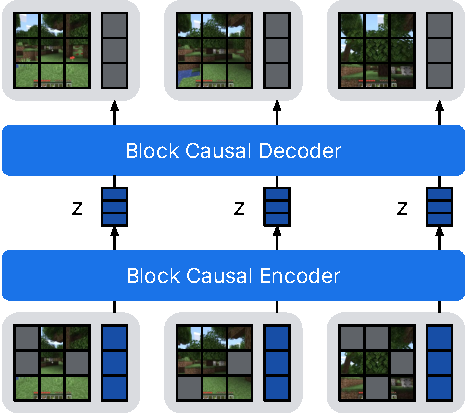
\includegraphics[height=2.4in]{figures/method/tok}
\caption{Causal Tokenizer}
\end{subfigure}%
\hfill%
\begin{subfigure}[t]{0.45\textwidth}
\centering
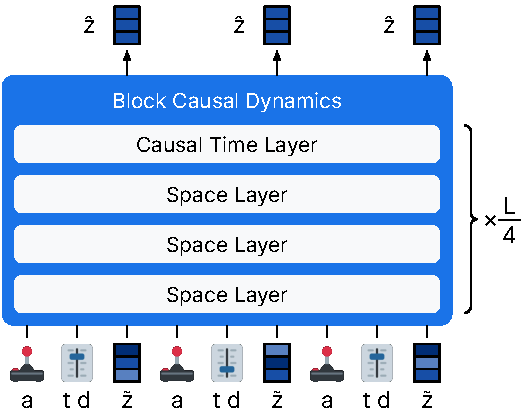
\includegraphics[height=2.5in]{figures/method/dyn}
\caption{Interactive Dynamics}
\end{subfigure}
\caption{World model design.
\method consists of a causal tokenizer and an interactive dynamics model, which both use the same block-causal transformer architecture.
The tokenizer encodes partially masked image patches and latent tokens, squeezes the latents through a low-dimensional projection with tanh activation, and decodes the patches.
It uses causal attention to achieve temporal compression while allowing frames to be decoded one by one.
The dynamics model operates on the interleaved sequence of actions, shortcut noise levels and step sizes, and tokenizer representations.
It denoises representations via a shortcut forcing objective.
After pretraining, the world model is finetuned into an agent by inserting task tokens into the dynamics transformer and predicting actions, rewards, and values from them.
}
\label{fig:model}
\end{figure}

We evaluate \method on the Minecraft diamond challenge, a long-horizon control task that requires solving several sub tasks, such as gathering materials and crafting tools in a complex procedurally generated 3D world from raw pixels and mouse and keyboard actions.
Human players with Minecraft experience take 20 minutes to collect a diamond on average, corresponding to sequences of 24,000 mouse and keyboard actions.

\paragraph{Offline setting}
While previous agents have achieved diamonds in Minecraft through online interaction with the environment \citep{vpt,dreamerv3}, deploying partially-trained policies is often infeasible for practical applications, such as physical robots, because ensuring safety, resetting the scene, and providing rewards in real time is difficult.
Instead, we focus on the challenge of learning purely offline from a fixed experience dataset.
We only use the VPT contractor dataset \citep{vpt}---which contains 2.5K hours of videos, actions, and event annotations---without allowing the agent to interact with the environment for learning, and compare to baselines in this offline setting.
We follow the VPT evaluation protocol of raw pixel inputs and low-level mouse and keyboard actions, requiring crafting through the in-game user interface.
Episodes last 60 minutes, starting from an empty inventory in randomly generated Minecraft worlds.

\paragraph{Implementation}
\method learns a single transformer that predicts inputs, actions, rewards, and values.
To build a steerable agent, we opt for a multi-task setting and condition the actions, rewards, and values on task embeddings.
We annotate the tasks and their sparse binary rewards using the existing events in the VPT dataset.
\Cref{tab:mc_tasks} lists the 20 tasks and \cref{tab:mc_ladder} shows the linear prompt sequence that guides the agent to reach diamonds during evaluation in the environment.
To amplify the signal in the dataset during behavior cloning, reward modeling, and reinforcement learning, we use data mixture of 50\% uniform sequences and 50\% relevant sequences that accomplish one of the tasks.
The behavioral cloning loss is applied only on the relevant fraction, while the dynamics loss is applied only on the uniform sequences to avoid optimistic generations.
We use one-hot task indicators but text embeddings could easily be used.
We represent keyboard actions as 23 binary distributions and mouse actions as a categorical with 121 classes using foveated discretization \citep{vpt}.

\pagebreak
We compare the following agents:

\begin{itemize}
\item\textbf{VPT (finetuned)}\quad
The strongest Minecraft agent for mouse and keyboard control in the literature\citep{vpt}.
The VPT paper presents two unconditioned behavioral cloning policies in the offline setting, both trained on 270K hours of synthetically annotated YouTube gameplay videos, and one further finetuned on a filtered subset of ``early game'' data.
We use the finetuned policy because it significantly outperforms the pretraining policy.

\item\textbf{BC (notask)}\quad
Behavioral cloning from scratch using multi-token prediction (MTP), without task conditioning.
While VPT uses the contractor data to train an action labeler and trains the policy on annotated YouTube videos, our BC agent trains directly and only on the relevant subset of the contractor actions.
This agent is not task conditioned, making it directly comparable to VPT.

\item\textbf{BC}\quad
Behavioral cloning from scratch on the filtered contractor dataset with task conditioning.
This agent is trained on the same filtered contractor dataset as BC (notask) but the additional task input makes it steerable.
When evaluating in the environment, the prompt sequence guides the agent through intermediate tasks towards mining diamonds.

\item\textbf{VLA (Gemma 3)}\quad
Following the VLA recipe \citep{kim2024openvla,intelligence2025pi05}, we train a behavioral cloning policy by finetuning the vision-language model Gemma 3\citep{team2025gemma3} on the relevant sequences using MTP.
Gemma 3 has been pretrained using substantially more compute and data than our other models, including native pretraining on images for visual perception, making it a strong baseline.

\item\textbf{WM+BC}\quad
The behavioral cloning policy of \method, before applying imagination training.
This policy is initialized from the world model pretrained on the full contractor dataset.
It then undergoes agent finetuning using behavioral cloning, reward modeling, and dynamics losses.

\item\textbf{Imagination RL}\quad
The full \method agent produced by finetuning the WM+BC agent through reinforcement learning in imagination, which we refer to as imagination training.
Despite performing on-policy reinforcement learning inside of the world model, there is no actual environment interaction, making it an offline method.
\end{itemize}

\begin{figure}[t!]
\vspace*{-2\baselineskip}
\centering
\begin{subfigure}[t]{0.45\textwidth}
\centering
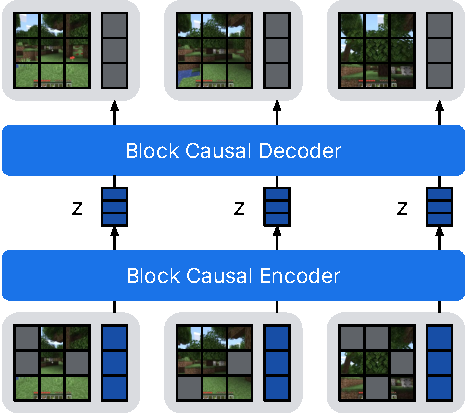
\includegraphics[height=2.4in]{figures/method/tok}
\caption{Causal Tokenizer}
\end{subfigure}%
\hfill%
\begin{subfigure}[t]{0.45\textwidth}
\centering
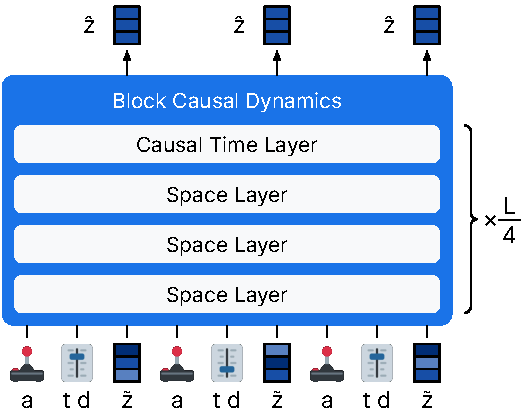
\includegraphics[height=2.5in]{figures/method/dyn}
\caption{Interactive Dynamics}
\end{subfigure}
\caption{World model design.
\method consists of a causal tokenizer and an interactive dynamics model, which both use the same block-causal transformer architecture.
The tokenizer encodes partially masked image patches and latent tokens, squeezes the latents through a low-dimensional projection with tanh activation, and decodes the patches.
It uses causal attention to achieve temporal compression while allowing frames to be decoded one by one.
The dynamics model operates on the interleaved sequence of actions, shortcut noise levels and step sizes, and tokenizer representations.
It denoises representations via a shortcut forcing objective.
After pretraining, the world model is finetuned into an agent by inserting task tokens into the dynamics transformer and predicting actions, rewards, and values from them.
}
\label{fig:model}
\end{figure}

\paragraph{Agent performance}
\Cref{fig:rl} compares the agent performance on the diamond task.
We report the success rates for several relevant items leading up to diamonds that are listed in \cref{tab:mc_items}.
VPT (finetuned) progresses up to sticks, which it achieves 53\% of the time.
It also collects a small amount of stone, iron ore, and iron ingots through edge cases, such as exploding Creeper mobs and loot chests.
Using the contractor actions directly instead of annotating YouTube videos, our modern BC baseline achieves higher performance than VPT (finetuned).
VLA (Gemma 3) shows that initializing the policy from a pretrained models offers significant benefits, progressing up to the iron pickaxe with a success rate of 11\%.
\method achieves high success rates of over 90\% up to the stone pickaxe, a success rate of 29\% for the iron pickaxe, and obtains diamonds in 0.7\% of episodes.
Imagination training shows stronger improvements over the behavior cloning agents the more challenging the milestone is.
\Cref{fig:rlabl} compares additional agents on the diamond task, showing that the world model representations outperform the general representations of Gemma 3 for behavioral cloning.
This indicates that video prediction implicitly learns an understanding of the world that is also useful for decision making.
Finally, imagination training consistently improves not only the success rates but also makes the policy more efficient so that it reaches the milestones faster.

\subsection{Human Interaction}
\label{sec:interact}

To evaluate its ability to predict complex interactions, we train \method on the Minecraft VPT dataset \citep{vpt} and compare its generations to previous world models on this dataset.
For this evaluation, a human player tries to accomplish tasks by playing inside of the world model, as shown in \cref{fig:wmtask}.
The human player receives the task description and the world model is initialized to a start frame for the task.
We select a diverse set of tasks that cover a broad range of object interactions and game mechanics.
The tasks include digging a pit, building a wall, chopping a tree, placing and riding a boat, looking away and back at objects, interacting with crafting benches and furnaces, and more.
We compare \method to the world models Oasis \citep{oasis}, Lucid-v1 \citep{lucidv1}, and MineWorld \citep{mineworld}.
Note that we cannot directly compare to Genie 3 \citep{genie3}, because it only supports camera actions and one generic ``interact'' button, whereas Minecraft requires a more general mouse and keyboard action space.
\Cref{tab:inference} summarizes the compared models.
Full results are given in \cref{fig:wmtasks_ours,fig:wmtasks_oasis,fig:wmtasks_lucid}.

\begin{table}[t!]
\centering
\begin{mytabular}{
  colspec = {| L{8em} | C{5em} C{5em} C{5em} C{5em} C{5em} |},
  row{1} = {font=\bfseries},
  stretch=0.9,
}

\toprule
Model & Parameters & Resolution & Context & FPS & Success \\
\midrule
MineWorld       & 1.2B & 384$\times$224 & 0.8s & \o\o2 & --- \\
Lucid-v1        & 1.1B & 640$\times$360 & 1.0s &  \o44 & 0/16 \\
Oasis (small)   & 500M & 640$\times$360 & 1.6s &  \o20 & 0/16 \\
Oasis (large)   & --- & 360$\times$360 & 1.6s &  \o\o\llap{$\sim$}5 & 5/16 \\
\midrule
\method         & 2B & 640$\times$360 & 9.6s &  \o21 & \textbf{14/16}  \\
\bottomrule

\end{mytabular}
\caption{
Comparison of Minecraft world models.
\method is the first world model to accurately simulate a wide range of object interactions and game mechanics in Minecraft.
Moreover, \method pushes the limits of context length compared to previous models by 6$\times$, while maintaining real-time interactive inference.
We measure the inference speed of each model on a single H100 GPU, and translate the inference speed for the proprietary large Oasis model based on public information.
The Minecraft dataset is recorded at 20 FPS, matching the update rate of the game.
}
\label{tab:inference}
\end{table}


\pagebreak
\paragraph{Inference speed}

We measure the inference speed of each model on  a single H100 GPU.
\method and Lucid-v1 achieve real-time interactive inference by exceeding the 20 FPS of the Minecraft physics engine\footnote{\url{https://minecraft.fandom.com/wiki/Tick}} and the VPT dataset \citep{vpt}.
\method has a substantially longer context of 9.6 seconds compared to the 0.8--1.6 seconds of prior models.
Oasis comes in two sizes, a 500M parameter version with open weights and a larger model of unknown size that is playable on the project website.
The small model achieves 20 FPS on one H100.
The large model is hosted on multiple H100s for interaction online and we estimate its inference speed on a single H100 around 5 FPS based on public information.
MineWorld achieves 2 FPS with their parallel decoding approach and is even slower without.
Additionally, parallel decoding requires knowing actions in advance, which is also required in the provided user interface.
Thus, it does not support real-time interactions and we cannot evaluate it on our tasks, which require many hundreds of actions.

\begin{figure}[t!]
\vspace*{-2\baselineskip}
\centering
\begin{subfigure}[t]{0.45\textwidth}
\centering
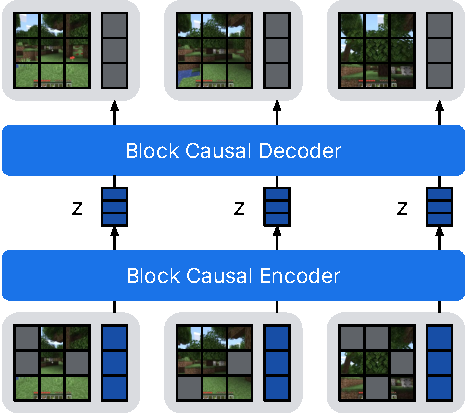
\includegraphics[height=2.4in]{figures/method/tok}
\caption{Causal Tokenizer}
\end{subfigure}%
\hfill%
\begin{subfigure}[t]{0.45\textwidth}
\centering
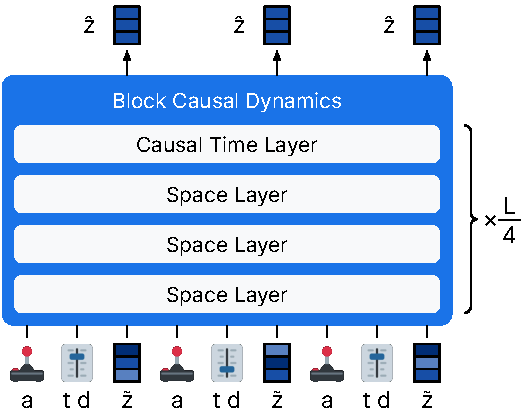
\includegraphics[height=2.5in]{figures/method/dyn}
\caption{Interactive Dynamics}
\end{subfigure}
\caption{World model design.
\method consists of a causal tokenizer and an interactive dynamics model, which both use the same block-causal transformer architecture.
The tokenizer encodes partially masked image patches and latent tokens, squeezes the latents through a low-dimensional projection with tanh activation, and decodes the patches.
It uses causal attention to achieve temporal compression while allowing frames to be decoded one by one.
The dynamics model operates on the interleaved sequence of actions, shortcut noise levels and step sizes, and tokenizer representations.
It denoises representations via a shortcut forcing objective.
After pretraining, the world model is finetuned into an agent by inserting task tokens into the dynamics transformer and predicting actions, rewards, and values from them.
}
\label{fig:model}
\end{figure}

\enlargethispage{2\baselineskip}
\paragraph{Complex interactions}

Video generations of human players attempting all tasks inside of the world models are shown in \cref{fig:wmtasks_ours,fig:wmtasks_oasis,fig:wmtasks_lucid}.
Lucid-v1 does not allow completing the tasks, with generations diverging or object interactions being ignored.
The large Oasis model allows performing 5 out of 16, such as placing torches, filling a window with glass panes, and opening a door.
However, it fails at building tasks because after placing a few blocks, it quickly hallucinates large structures into the world.
This ``autocompletion'' failure mode reflects a lack of understanding of the game mechanics.
We did not evaluate MineWorld because of its lack of interactive inference.
\method achieves 14 out of 16 tasks, accurately generating complex interactions and game mechanics such as switching items, placing and breaking blocks, fighting monsters, placing and riding boats, entering portals, and more.
Its temporal consistency is limited to a context of 9.6 seconds, albeit substantially longer than previous models.
While it correctly generates the interfaces for inventory, crafting, and furnaces and predicts most mouse movement, inventory items are sometimes unclear or change over time, leaving room for future improvements.

As a step towards testing the applicability of \method to real world video, we also train the world model on a robotics dataset\citep{soar}.
In \cref{fig:robotics}, we observe accurate physics and counterfactual interactions with real world objects, overcoming the causal confusion of existing video models.
Additional details are included in the supplementary material.

\subsection{Action Generalization}
\label{sec:actgen}

One promise of world models is to leverage diverse unlabeled videos to teach agents about the world.
For example, a world model could learn general physics and object interactions from web videos where actions are not available.
In this section, we investigate the amount of paired videos with actions that are needed for grounding an embodiment into the \method world model.
Intuitively, the world model has to learn a broader distribution of possible outcomes when actions are missing, and can narrow the distribution down when actions are provided.
Moreover, we investigate how well the action conditioning generalizes, not just within the same distribution, but also out of distribution to parts of the world specifically held out.
To measure the accuracy of the action conditioning, we compare action-conditioned multi-step generations to ground truth videos on the holdout set.
We report PSNR and SSIM for 16-step generations given 320 frames of context.

\begin{figure}[t!]
\vspace*{-2\baselineskip}
\centering
\begin{subfigure}[t]{0.45\textwidth}
\centering
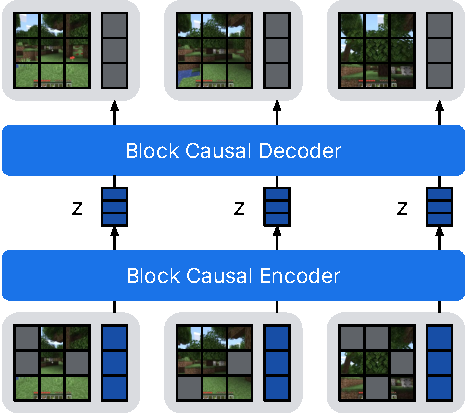
\includegraphics[height=2.4in]{figures/method/tok}
\caption{Causal Tokenizer}
\end{subfigure}%
\hfill%
\begin{subfigure}[t]{0.45\textwidth}
\centering
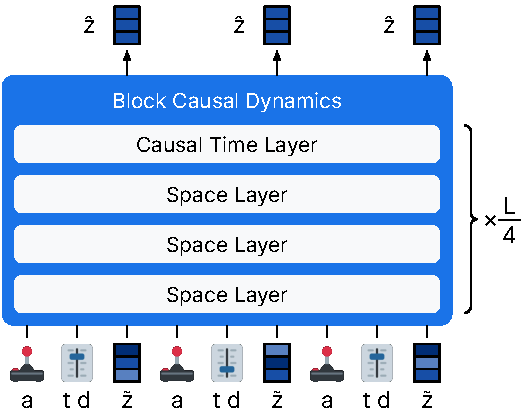
\includegraphics[height=2.5in]{figures/method/dyn}
\caption{Interactive Dynamics}
\end{subfigure}
\caption{World model design.
\method consists of a causal tokenizer and an interactive dynamics model, which both use the same block-causal transformer architecture.
The tokenizer encodes partially masked image patches and latent tokens, squeezes the latents through a low-dimensional projection with tanh activation, and decodes the patches.
It uses causal attention to achieve temporal compression while allowing frames to be decoded one by one.
The dynamics model operates on the interleaved sequence of actions, shortcut noise levels and step sizes, and tokenizer representations.
It denoises representations via a shortcut forcing objective.
After pretraining, the world model is finetuned into an agent by inserting task tokens into the dynamics transformer and predicting actions, rewards, and values from them.
}
\label{fig:model}
\end{figure}

\paragraph{Amount of actions}
To understand the amount of video with actions needed to learn action conditioning, we train \method on all 2541 hours of videos in the VPT dataset, but only provide actions for a small subset of the videos.
When actions are unavailable, the dynamics model is conditioned on a learned embedding, as described in \cref{sec:dynamics}.
We train \method models with 0, 10, 100, 1000, and 2541 hours of actions.
The available actions are the first in sequential order of the dataset, corresponding to fewer unique worlds and players than random shuffling would yield.
\Cref{fig:actgen} show the quality of the action conditioning compared to training with no actions at all to training with all actions.
With only 10 hours of actions, \method achieves 53\% PSNR and 75\% SSIM compared to a model trained with all actions.
With 100 hours of actions, the performance increases further to 85\% PSNR and 100\% SSIM.
This result demonstrates that world models absorb the majority of their knowledge from unlabeled videos, and require only a small amount of actions.

\paragraph{Action extrapolation}

In principle, world models may not only learn action ground from a few actions but also generalize their action conditioning to completely new scenarios.
In the future, this could allow world models to absorb general knowledge from diverse web videos to simulate agents in diverse environments.
We perform, to the best of our knowledge, the first controlled evaluation of this hypothesis.
For this, we carefully split the VPT dataset into one portion that only contains videos of the Overworld and another portion that only contains the other two game dimensions, the Nether and End.
Where the Overworld contains forests, deserts, oceans, and more, the Nether and End feature substantially different and unique visuals.
The Nether is an underworld filled with lava and red blocks and the End is filled with yellow blocks and black towers unseen in the Overworld.
We train \method on videos of both datasets but only provide actions for the Overworld.
We then perform an action-conditioned evaluation of the resulting model on the Nether and End, for which it has never seen any actions.
In a prior experiment, we observed that training only on the Overworld portion without any Nether videos results in poor generation scores for Nether start frames.
\Cref{fig:actgen} reports the relative performance compared to training without any or with all actions.
Surprisingly, the world model achieves 76\% of the PSNR and 80\% of the SSIM of the model trained with all actions.
This demonstrates that the action conditioning of world models can generalize to scenarios known only from unlabeled videos.

\subsection{Model Design}
\label{sec:modeldesign}

\begin{table}[tb!]
\centering
\vspace*{-2ex}
\begin{mytabular}{
  colspec = {| L{15em} | C{5.5em} C{5.5em} C{5.5em} |},
  row{1} = {font=\bfseries},
  stretch=0.9,
}

\toprule
Model & Train step seconds & Inference FPS (\rlap{$\uparrow$)} & Quality FVD (\rlap{$\downarrow$)} \\
\midrule

Diffusion Forcing Transformer               & 9.8 & \o0.8 &  306 \\  % model1
+ Fewer sampling steps ($K=4$)              & 9.8 & \o9.1 &  875 \\  % model1
+ Shortcut model                            & 9.8 & \o9.1 &  329 \\  % model2
+ X-Prediction                              & 9.8 & \o9.1 &  326 \\  % model3
+ X-Loss                                    & 9.8 & \o9.1 &  151 \\  % model4
+ Ramp weight                               & 9.8 & \o9.1 &  102 \\  % model5
+ Alternating batch lengths                 & 1.5 & \o9.1 & \o80 \\  % model6
+ Long context every 4 layers               & 0.6 &  18.9 & \o70 \\  % model7
+ GQA                                       & 0.5 &  23.2 & \o71 \\  % model8
+ Time factorized long context              & 0.4 &  30.1 & \o91 \\  % model9
+ Register tokens                           & 0.5 &  28.9 & \o91 \\  % model10
+ More spatial tokens ($N_\mathrm{z}=128$)  & 0.8 &  25.7 & \o66 \\  % model11
+ More spatial tokens ($N_\mathrm{z}=256$)  & 1.7 &  21.4 & \o57 \\  % model12
\bottomrule

% Ours with vpred: 123.75

\end{mytabular}
\caption{
Cascade of model design choices.
\method is based on a shortcut forcing objective and an efficient transformer architecture, combining a range of known techniques to achieve accurate and fast interleaved generation.
Starting from a naive diffusion forcing transformer with $N_\mathrm{z}=64$ spatial tokens and $K=64$ sampling steps, we apply the objective and architecture modifications, and increase the number of spatial tokens once feasible.
Inference speed measured on a single H100 GPU.
The resulting world model achieves high model capacity and inference efficiency.
}
\label{tab:ablations}
\end{table}


World models require high model capacity to predict complex object interactions and fast inference to support imagination training and human interaction for inspection.
Moreover, interactive inference prompts different design choices compared to typical video models to enable fast generation of individual frames and prevent accumulating errors.
In this section, we ablate the objective and architecture decisions of \method by applying a cascade of improvements to a naive diffusion forcing transformer baseline.
To evaluate each model, we train for 48 hours and then generate 1024 videos of 384 frames (\~20 seconds) each without any context, with interactive actions chosen by a fixed behavioral cloning policy.
We then split the resulting videos into 16 frame chunks to compute the Frech\'et Video Distance (FVD) \citep{fvd} to the holdout dataset.

\pagebreak
\begin{figure}[t!]
\vspace*{-2\baselineskip}
\centering
\begin{subfigure}[t]{0.45\textwidth}
\centering
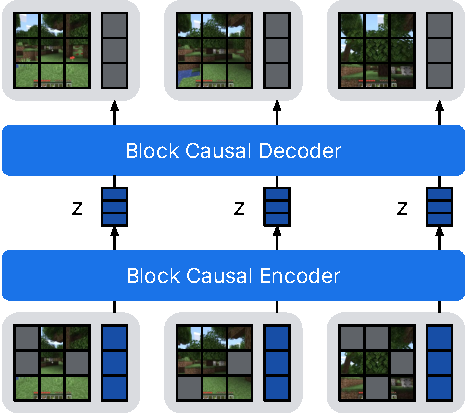
\includegraphics[height=2.4in]{figures/method/tok}
\caption{Causal Tokenizer}
\end{subfigure}%
\hfill%
\begin{subfigure}[t]{0.45\textwidth}
\centering
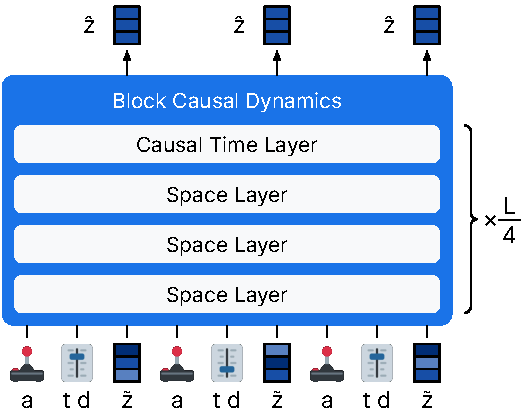
\includegraphics[height=2.5in]{figures/method/dyn}
\caption{Interactive Dynamics}
\end{subfigure}
\caption{World model design.
\method consists of a causal tokenizer and an interactive dynamics model, which both use the same block-causal transformer architecture.
The tokenizer encodes partially masked image patches and latent tokens, squeezes the latents through a low-dimensional projection with tanh activation, and decodes the patches.
It uses causal attention to achieve temporal compression while allowing frames to be decoded one by one.
The dynamics model operates on the interleaved sequence of actions, shortcut noise levels and step sizes, and tokenizer representations.
It denoises representations via a shortcut forcing objective.
After pretraining, the world model is finetuned into an agent by inserting task tokens into the dynamics transformer and predicting actions, rewards, and values from them.
}
\label{fig:model}
\end{figure}%
\Cref{tab:ablations} shows the progression of models and their generation quality and speed.
We start with a standard block-causal transformer with dense attention and diffusion forcing with velocity parameterization.
We target 20 FPS interactive inference on a single H100 GPU, matching the tick rate of Minecraft and the framerate of the VPT dataset.
With 64 sampling steps per frame, the baseline falls short of real-time generations with only 0.8 FPS on one H100 GPU, while 4 sampling steps achieve 9.1 FPS but result in poor quality.
Shortcut models \citep{shortcut} nearly recover the original visual quality with only 4 sampling steps.
We then parameterize the model to make x-space predictions, compute the loss in x-space, and apply the ramp loss weight.
These changes substantially improve generation quality over traditional v-space prediction, especially for long generations.
We hypothesize that the prediction targets in x-space are more structured and thus reduce the risk of high-frequency errors that accumulate over time.
\Cref{fig:nfe} compares the visual quality of shortcut forcing to diffusion forcing---both using the x-space loss with ramp weight---for a wider range of sampling steps.

Training on alternating batch lengths is similar to progressive training and speeds up learning while allowing to generate long videos for inspection throughout training.
Using temporal attention only every 4 layers not only speeds up training and inference \citep{llama4} but also improves generation quality, possibly because of the inductive bias of spatial attention that focuses computation on the current frame.
GQA further accelerates generations without degrading performance.
Switching the long context layers from dense to time-only attention accelerates inference at a mild quality cost, and prepares us to increase the overall number of tokens subsequently.
While the register tokens do not improve FVD measurably, we qualitatively notice that they improve temporal consistency.
After these changes, training and inference is fast enough to increase model capacity through more spatial tokens, improving predictions of complex interactions.
The complete model achieves an FVD of 57 compared to 306 for the naive diffusion forcing transformer baseline and 124 for the complete architecture with v-space prediction and losses.

\vfill
\begin{table}[h!]
\centering
\begin{mytabular}{
  colspec = {| L{6em} | C{5em} C{9em} | C{3.5em} C{3.5em} C{3.5em} |},
  row{1} = {font=\bfseries},
  stretch = 0.9,
}

\toprule
\SetCell[r=2]{m}{Agent} &
\SetCell[r=2]{m}{Inputs} &
\SetCell[r=2]{m}{Actions} &
\SetCell[c=3]{c}{Data (hours)} \\
& & & Offline & Web & Online \\

\midrule
{Dreamer 3} & {64$\times$64,\\inventory} & {keyboard, camera,\\ abstract crafting} & --- & --- & 1.4K \\[1ex]
VPT (RL) & 128$\times$128 & {keyboard, mouse} & 2.5K & 270K & 194K \\[1ex]
VPT (BC) & 128$\times$128 & {keyboard, mouse} & 2.5K & 270K & --- \\[1ex]
\method & 360$\times$640 & {keyboard, mouse} & 2.5K & --- & --- \\
\bottomrule

\end{mytabular}
\caption{
Comparison of experimental setups for different Minecraft agents.
\method learns purely from offline experience and requires 100$\times$ less data than previous keyboard and mouse agents.
See \cref{fig:inputs} for examples of input images.
}
\label{tab:setups}
\end{table}


\pagebreak
\section{Related Work}

\paragraph{Minecraft agents}

Obtaining diamonds in the video game Minecraft has been a focus of intelligent agent research \citep{johnson2016malmo,guss2019minerl,kanervisto2022minerlcomp,kanitscheider2021minecraftcurriculum}, a long-horizon task that requires gathering resources and crafting tools through thousands of low-level actions in complex procedurally generated 3D worlds.
Different setups have been used in the literature, with \cref{tab:setups} summarizing the ones relevant to our work.
VPT \citep{vpt} collects 2.5K hours of contractor gameplay and uses it to annotate 270K hours of web videos with synthetic mouse and keyboard actions.
Behavioral cloning on this large offline dataset and targeted finetuning on ``early-game'' data yields a policy that occasionally obtains wooden pickaxes.
Following up with 194K hours of online reinforcement learning results in a policy that obtains diamonds and diamond pickaxes.
Dreamer 3 \citep{dreamerv3} learns to collect diamonds from scratch from 1.4K hours of online interaction, without any human data.
It uses the MineRL competition action space that includes abstract crafting actions.
Other works have explored novel algorithms for easier tasks\citep{lifshitz2023steve1,cai2023minecraftgroot,zhou2024minedreamer,nieto2021minecraftskills}.
In this paper, we train an agent to achieve diamonds purely from the 2.5K hour contractor dataset, without any online interaction.
We use low-level mouse and keyboard actions and high-resolution image inputs.

\paragraph{World model agents}

Learning behaviors based on learned models of the environment has been explored for a long time \citep{sutton1991dyna,deisenroth2011pilco,watter2015e2c}.
Visual Foresight \citep{finn2017visualforesight}, the work by \citet{ha2018worldmodels}, and PlaNet \citep{hafner2018planet} achieved world models accurate enough for planning from pixels.
With Dreamer, world models have become the state-of-the-art approach for solving control problems with high-dimensional inputs, outperforming model-free reinforcement learning in robustness, efficiency, and final performance \citep{hafner2019dreamer,hafner2020dreamerv2,dreamerv3}.
World models based on transformers or diffusion objectives have demonstrated high data efficiency for discrete control \citep{micheli2022iris,robine2023twm,storm}.
However, these world models have been limited in model capacity, restricting their applicability to relatively simple simulated environments.

\paragraph{Scalable world models}

Larger world models have been shown to simulate more complex data distributions \citep{yu2025survey}.
World models like Genie 3 generate highly diverse scenes and simulate camera movement and simple interactions\citep{genie3,he2025matrix,sun2025virtual,team2025yan}.
PlayerOne\citep{tu2025playerone} and PEVA\citep{bai2025whole} condition on more detailed human movement.
Oasis \citep{oasis}, Lucid \citep{lucidv1}, and MineWorld \cite{mineworld} learn Minecraft simulators from mouse and keyboard inputs.
Whereas Oasis captures simple game mechanics and achieves real-time inference on specialized hardware, Lucid's predictions diverge quickly and MineWorld is slower than real time.
GameNGen \citep{valevski2024diffusion} finetunes Stable Diffusion into a playable simulator of a level of the game Doom.
DIAMOND \citep{alonso2024diffusion} learns a simulator of a level of the game CS GO, achieving short-term predictions.
GAIA \citep{hu2023gaia,russell2025gaia} generates driving scenarios from real world data.
However, these world models still struggle to predict complex object interactions precisely enough for imagination training.

\paragraph{Fast generation}

Enabling fast and accurate generations has been a long-standing challenge in generating modeling.
MaskGit generates discrete tokens in parallel to accelerate sampling over autoregressive models \citep{chang2022maskgit}.
Diffusion models are often distilled to enable sampling using fewer forward passes \citep{salimans2022progressive,kodaira2025streamdit}, which requires two training phases.
Consistency models learn straight paths to enable fast image generation but require careful schedules \citep{song2023consistency,song2023improved,lu2024simplifying}, with successful applications to video generation \citep{wang2023videolcm}.
Shortcut models \citep{shortcut} condition flows on both noise level and step size, producing fast generative models in one training phase and without schedules.
Mean Flow \citep{geng2025meanflow} extends the idea of conditioning on the step size to a continuous time formulation.
Efficient and sparse architectures are used for video generation because of the large number of tokens \citep{axial,zhao2024real,zhang2025vsa}.
These models do not support interactive inference and many of the techniques are complimentary to our work.

\section{Discussion}

We present \method, a scalable agent that learns to solve challenging control tasks by imagination training inside of a fast and accurate world model.
\method is the first agent to obtain diamonds in Minecraft purely from offline data, without online interaction.
This achievement demonstrates its learning successful long-horizon strategies in complex environments.
Learning purely from offline datasets enables applications where online interaction is impractical or unsafe.

The world model of \method rests on a shortcut forcing objective and an efficient transformer architecture to predict complex object interactions while supporting interactive inference in real time on a single GPU.
We demonstrate that it significantly outperforms previous world models on Minecraft, where it accurately predicts a wide range of game mechanics from mouse and keyboard inputs.
However, the world model is far from a full clone of the game, especially due to short memory and imprecise inventory predictions, leaving Minecraft as an ideal benchmark for future world model and agent research.
We also show that \method learns accurate action conditioning from only a small amount of videos with actions, allowing it to absorb the majority of its knowledge from diverse unlabeled videos.

Promising future directions include pretraining on general internet videos, integrating long-term memory into the world model and agent, incorporating language understanding, leveraging small amounts of corrective online data, and automatically discovering goals to break up long tasks.
\method offers a reliable and performant starting point for these explorations.

\clearpage
\begin{hyphenrules}{nohyphenation}
\setlength{\bibsep}{.5ex plus .5ex}
\bibliography{references}
\end{hyphenrules}

\clearpage
\appendix
% \section{Supplementary Material}

\section{Datasets}

\paragraph{Minecraft VPT}

We use the OpenAI VPT dataset of contractor gameplay \citep{vpt} and combine the available subsets 6--10, resulting in 2541 hours of gameplay.
We split the dataset into 90\% training and 10\% evaluation data, ensuring that the splits do not share any of the same underlying 5-min recording chunks.
We encode keyboard actions as a vector of binary variables and process the mouse actions as in VPT by $\mu$-law encoding, discretizing into 11 bins per coordinate, and enumerating all $11 \times 11 = 121$ combinations to obtain a categorical variable.
The image resolution is $360 \times 640$ and the framerate is 20 FPS.
We zero pad the frames to $384 \times 640$ and then patchify with patch size $16 \times 16$ into 960 tokens.
We reshape the $(N_\mathrm{b} = 512) \times (D_\mathrm{b} = 16)$ bottleneck of the tokenizer to $(N_\mathrm{z} = 256) \times 32$ for the dynamics model.
We train the dynamics model with $N_\mathrm{z} = 256$ spatial tokens, context length $C = 192$, and batch lengths $T_1 = 64$ and $T_2 = 256$.

\paragraph{Minecraft Overworld and Nether split}

To study out-of-distribution generalization of action conditioning in \method, we carefully split the Minecraft dataset into videos of the Overworld versus the Nether dimension.
We also include the End dimension into the Nether portion of the dataset.
Both the Nether and the End feature unique visuals, blocks, and terrain shapes compared to the Overworld.
The Overworld includes natural landscapes with forests, deserts, oceans, and more, whereas the Nether is underworld-themed with red blocks and lava and the End is a space-themed region.
To separate the dataset, we want to ensure no leakage from players entering the Nether/End dimensions and bringing blocks from there back to the Overworld.
For this reason, we exclude the VPT 6 and 7 subsets, which contain long free play.
We then assigned each 5 min recording of the remaining dataset to either the Overworld or the Nether/End portion based on item events that are provided by the dataset.
Whenever a Nether/End item was interacted with, we assign that video to the Nether/End split.
This ensures that the Overworld split contains no Nether/End episodes, whereas the Nether/End split can sometimes contain some Overworld episodes, although this was rare in practice.
We manually investigated the Overworld split obtained by this strategy and found no Nether/End trajectories in it.

\paragraph{SOAR Robotics}

The SOAR dataset \citep{soar} contains teleoperated demonstrations and online trajectories of a reinforcement learning policy, thus covering both successes and failures.
We split the dataset into 90\% training and 10\% evaluation data.
The dataset contains a total of 180 hours of videos with 7D relative end-effector actions.
The image resolution is $256 \times 256$ and the framerate is 5 FPS.
We patchify with patch size $16 \times 16$ into 256 tokens.
We train the dynamics model with $N_\mathrm{z} = 512$ spatial tokens, context length $C = 96$, and batch lengths $T_1 = 32$ and $T_2 = 128$.

\paragraph{Epic Kitchens}

The Epic Kitchens 100 dataset \citep{epickitchens} contains 100 hours of video from the first-person perspective of humans across 45 kitchens.
The test set contains different tasks performed in the same kitchens.
We use the dataset at $256 \times 256$ resolution and 10 FPS.
We patchify with patch size $16 \times 16$ into 256 tokens.
We train the dynamics model with $N_\mathrm{z} = 512$ spatial tokens, context length $C = 96$, and batch lengths $T_1 = 32$ and $T_2 = 128$.

\clearpage
\section{Kitchen Generations}
\vfill
\begin{figure}[t!]
\vspace*{-2\baselineskip}
\centering
\begin{subfigure}[t]{0.45\textwidth}
\centering
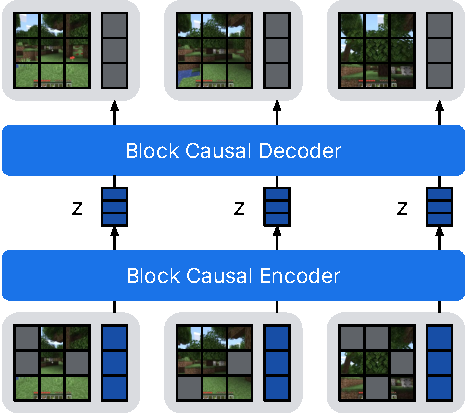
\includegraphics[height=2.4in]{figures/method/tok}
\caption{Causal Tokenizer}
\end{subfigure}%
\hfill%
\begin{subfigure}[t]{0.45\textwidth}
\centering
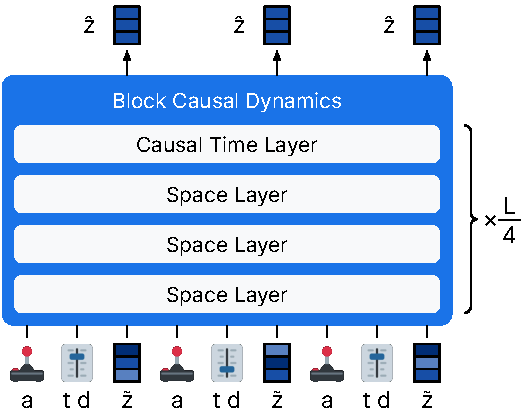
\includegraphics[height=2.5in]{figures/method/dyn}
\caption{Interactive Dynamics}
\end{subfigure}
\caption{World model design.
\method consists of a causal tokenizer and an interactive dynamics model, which both use the same block-causal transformer architecture.
The tokenizer encodes partially masked image patches and latent tokens, squeezes the latents through a low-dimensional projection with tanh activation, and decodes the patches.
It uses causal attention to achieve temporal compression while allowing frames to be decoded one by one.
The dynamics model operates on the interleaved sequence of actions, shortcut noise levels and step sizes, and tokenizer representations.
It denoises representations via a shortcut forcing objective.
After pretraining, the world model is finetuned into an agent by inserting task tokens into the dynamics transformer and predicting actions, rewards, and values from them.
}
\label{fig:model}
\end{figure}
\vfill

\section{Minecraft Tasks}
\vspace*{-2ex}
\begin{minipage}[t]{0.48\textwidth}
\centering
\vspace*{1ex}
\begin{mytabular}{
  colspec = {| C{3em} | L{13em} |},
  row{1} = {font=\bfseries},
}

\toprule
Index & Task \\
\midrule
  1 & \texttt{mine\_log} \\
  2 & \texttt{mine\_cobblestone} \\
  3 & \texttt{mine\_iron\_ore} \\
  4 & \texttt{mine\_coal} \\
  5 & \texttt{mine\_diamond} \\
  6 & \texttt{craft\_planks} \\
  7 & \texttt{craft\_stick} \\
  8 & \texttt{craft\_crafting\_table} \\
  9 & \texttt{craft\_furnace} \\
 10 & \texttt{craft\_iron\_ingot} \\
 11 & \texttt{craft\_wooden\_pickaxe} \\
 12 & \texttt{craft\_stone\_pickaxe} \\
 13 & \texttt{craft\_iron\_pickaxe} \\
 14 & \texttt{open\_crafting\_table} \\
 15 & \texttt{open\_furnace} \\
 16 & \texttt{place\_crafting\_table} \\
 17 & \texttt{place\_furnace} \\
 18 & \texttt{use\_wooden\_pickaxe} \\
 19 & \texttt{use\_stone\_pickaxe} \\
 20 & \texttt{use\_iron\_pickaxe} \\
\bottomrule

\end{mytabular}
\captionof{table}{Taskset for training the multi-task agent.}
\label{tab:mc_tasks}

\vspace*{3ex}
\centering
\newcommand{\icon}[1]{\includegraphics[height=2.5ex]{icons/#1.png}}
\newcommand{\name}[1]{\raisebox{.4ex}{#1}}
\vspace*{1ex}
\begin{mytabular}{
  colspec = {| C{3em} | L{13em} |},
  row{1} = {font=\bfseries},
}

\toprule
Icon & Item \\
\midrule
\icon{log} & \name{Log} \\
\icon{planks} & \name{Planks} \\
\icon{stick} & \name{Stick} \\
\icon{crafting_table} & \name{Crafting table} \\
\icon{wooden_pickaxe} & \name{Wooden pickaxe} \\
\icon{cobblestone} & \name{Cobblestone} \\
\icon{stone_pickaxe} & \name{Stone pickaxe} \\
\icon{iron_ore} & \name{Iron ore} \\
\icon{furnace} & \name{Furnace} \\
\icon{iron_ingot} & \name{Iron ingot} \\
\icon{iron_pickaxe} & \name{Iron pickaxe} \\
\icon{diamond} & \name{Diamond} \\
\bottomrule

\end{mytabular}
\captionof{table}{Milestone items used for measuring progress during evaluation.}
\label{tab:mc_items}

\end{minipage}
\hfill%
\begin{minipage}[t]{0.48\textwidth}
\centering
\vspace*{1ex}
\begin{mytabular}{
  colspec = {| L{13em} | C{3em} |},
  row{1} = {font=\bfseries},
}

\toprule
Task & Count \\
\midrule

\texttt{mine\_log} & 10 \\
\texttt{craft\_planks} & 20 \\
\texttt{craft\_crafting\_table} & 1 \\
\texttt{place\_crafting\_table} & 1 \\
\texttt{craft\_stick} & 4 \\
\texttt{craft\_wooden\_pickaxe} & 1 \\
\texttt{use\_wooden\_pickaxe} & 1 \\
\texttt{mine\_cobblestone} & 3 \\
\texttt{craft\_planks} & 4 \\
\texttt{craft\_crafting\_table} & 1 \\
\texttt{place\_crafting\_table} & 1 \\
\texttt{craft\_stick} & 4 \\
\texttt{craft\_stone\_pickaxe} & 1 \\
\texttt{use\_stone\_pickaxe} & 1 \\
\texttt{mine\_iron\_ore} & 3 \\
\texttt{mine\_cobblestone} & 8 \\
\texttt{craft\_planks} & 4 \\
\texttt{craft\_crafting\_table} & 1 \\
\texttt{place\_crafting\_table} & 1 \\
\texttt{craft\_furnace} & 1 \\
\texttt{craft\_iron\_ingot} & 3 \\
\texttt{craft\_stick} & 2 \\
\texttt{craft\_iron\_pickaxe} & 1 \\
\texttt{use\_iron\_pickaxe} & 1 \\
\texttt{mine\_diamond} & $\infty$ \\

\bottomrule

\end{mytabular}
\captionof{table}{Prompt sequence for evaluation.}
\label{tab:mc_ladder}

\end{minipage}
\clearpage

\section{Offline Diamond Challenge}
\begin{table}[h!]
\centering
\newcommand{\rot}[1]{\hspace*{1ex}\rotatebox{70}{#1}}
\begin{mytabular}{
  colspec = {| L{8em} | C{3em} C{3em} C{3em} C{3em} C{3em} C{3em} C{3em} C{3em} |},
  row{1} = {font=\bfseries},
  stretch=0.9,
}
\toprule
Item & \rot{VPT (pretrained)} & \rot{VPT (finetuned)} & \rot{BC (notask)} & \rot{WM+BC (notask)} & \rot{BC} & \rot{VLA (Gemma 3)} & \rot{WM+BC} & \rot{Dreamer 4} \\
\midrule
Log            &           \o81.9  &           \o84.3  &           \o71.4  &           \o92.6  &   \textbf{\o97.3} &   \textbf{\o98.5} &   \textbf{\o99.6} &   \textbf{\o99.1} \\
Planks         &           \o30.6  &           \o65.3  &           \o68.6  &           \o91.6  &   \textbf{\o95.7} &   \textbf{\o98.3} &   \textbf{\o99.6} &   \textbf{\o98.9} \\
Crafting table &          \o\o1.7  &          \o\o4.7  &           \o63.8  &           \o90.6  &           \o93.5  &   \textbf{\o97.2} &   \textbf{\o99.1} &   \textbf{\o98.5} \\
Stick          &           \o30.3  &           \o52.6  &           \o62.4  &           \o90.1  &   \textbf{\o95.0} &   \textbf{\o97.7} &   \textbf{\o98.9} &   \textbf{\o98.7} \\
Wooden pickaxe &          \o\o0.0  &          \o\o0.0  &           \o33.8  &           \o77.3  &           \o86.5  &   \textbf{\o94.1} &   \textbf{\o97.3} &   \textbf{\o96.6} \\
Cobblestone    &          \o\o4.8  &          \o\o6.9  &           \o32.0  &           \o77.4  &           \o83.9  &           \o91.6  &   \textbf{\o97.2} &   \textbf{\o95.9} \\
Stone pickaxe  &          \o\o0.0  &          \o\o0.0  &          \o\o8.8  &           \o38.4  &           \o53.8  &           \o76.7  &   \textbf{\o89.4} &   \textbf{\o90.1} \\
Iron ore       &          \o\o0.1  &          \o\o0.1  &          \o\o3.6  &           \o22.0  &           \o26.5  &           \o46.3  &           \o62.9  &   \textbf{\o66.7} \\
Furnace        &          \o\o0.0  &          \o\o0.0  &          \o\o4.0  &           \o28.0  &           \o16.2  &           \o42.4  &           \o51.1  &   \textbf{\o58.1} \\
Iron ingot     &          \o\o0.1  &          \o\o0.1  &          \o\o0.2  &          \o\o1.2  &          \o\o4.3  &           \o22.5  &           \o27.8  &   \textbf{\o39.5} \\
Iron pickaxe   &          \o\o0.0  &          \o\o0.0  &          \o\o0.0  &          \o\o0.1  &          \o\o0.6  &           \o11.2  &           \o16.9  &   \textbf{\o29.0} \\
Diamond        &          \o\o0.0  &          \o\o0.0  &          \o\o0.0  &          \o\o0.0  &          \o\o0.0  &          \o\o0.0  &          \o\o0.0  &  \textbf{\o\o0.7} \\
\bottomrule
\end{mytabular}
\caption{Success rates for each milestone item averaged over 1000 evaluation episodes. Scores within 5\% of the highest recorded score are highlighted in bold.}
\label{tab:rl_success}
\end{table}

\begin{table}[h!]
\centering
\newcommand{\rot}[1]{\hspace*{1ex}\rotatebox{70}{#1}}
\begin{mytabular}{
  colspec = {| L{8em} | C{3em} C{3em} C{3em} C{3em} C{3em} C{3em} C{3em} C{3em} |},
  row{1} = {font=\bfseries},
  stretch=0.9,
}
\toprule
Item & \rot{VPT (pretrained)} & \rot{VPT (finetuned)} & \rot{BC (notask)} & \rot{WM+BC (notask)} & \rot{BC} & \rot{VLA (Gemma 3)} & \rot{WM+BC} & \rot{Dreamer 4} \\
\midrule
Log            &          \o\o9.1  &          \o\o6.3  &           \o11.9  &          \o\o5.4  &          \o\o1.8  &          \o\o2.2  &          \o\o1.2  &  \textbf{\o\o0.9} \\
Planks         &           \o25.2  &           \o14.2  &           \o12.2  &          \o\o5.9  &          \o\o4.3  &          \o\o3.4  &          \o\o2.1  &  \textbf{\o\o2.0} \\
Stick          &           \o32.0  &           \o24.0  &           \o13.3  &          \o\o6.7  &          \o\o6.4  &          \o\o5.0  &  \textbf{\o\o3.1} &  \textbf{\o\o2.9} \\
Crafting table &           \o41.4  &           \o27.5  &           \o17.1  &          \o\o8.0  &          \o\o9.5  &          \o\o7.2  &  \textbf{\o\o4.6} &  \textbf{\o\o4.4} \\
Wooden pickaxe &               --- &               --- &           \o18.8  &           \o11.6  &           \o11.4  &          \o\o9.8  &          \o\o5.7  &  \textbf{\o\o5.0} \\
Cobblestone    &               --- &               --- &           \o19.6  &           \o12.7  &           \o13.3  &           \o12.1  &          \o\o6.7  &  \textbf{\o\o5.6} \\
Stone pickaxe  &               --- &               --- &           \o23.5  &           \o15.7  &           \o15.8  &           \o14.5  &          \o\o8.9  &  \textbf{\o\o6.7} \\
Iron ore       &               --- &               --- &           \o28.9  &           \o17.5  &           \o20.9  &           \o23.5  &           \o14.3  &  \textbf{\o\o9.9} \\
Furnace        &               --- &               --- &           \o29.4  &           \o19.7  &           \o24.5  &           \o24.7  &           \o16.1  &   \textbf{\o11.0} \\
Iron ingot     &               --- &               --- &               --- &           \o30.5  &           \o28.8  &           \o30.8  &           \o17.2  &   \textbf{\o12.4} \\
Iron pickaxe   &               --- &               --- &               --- &               --- &           \o29.1  &           \o31.1  &           \o17.0  &   \textbf{\o13.3} \\
Diamond        &               --- &               --- &               --- &               --- &               --- &               --- &               --- &   \textbf{\o20.7} \\
\bottomrule
\end{mytabular}
\caption{Time in minutes needed for reaching each milestone item, averaged over successful episodes. We omit timings for items below a success rate of 0.5\% to ensure statistical significance. Scores within 5\% of the fastest recorded score are highlighted in bold.}
\label{tab:rl_timing}
\end{table}

\clearpage

\enlargethispage{\baselineskip}
\vspace*{-9ex}
\section{Minecraft Inputs}
\vspace*{-1ex}
\begin{figure}[t!]
\vspace*{-2\baselineskip}
\centering
\begin{subfigure}[t]{0.45\textwidth}
\centering
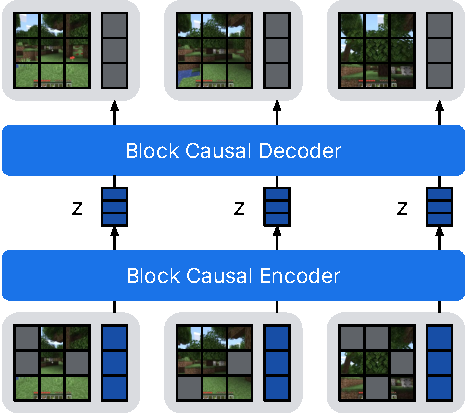
\includegraphics[height=2.4in]{figures/method/tok}
\caption{Causal Tokenizer}
\end{subfigure}%
\hfill%
\begin{subfigure}[t]{0.45\textwidth}
\centering
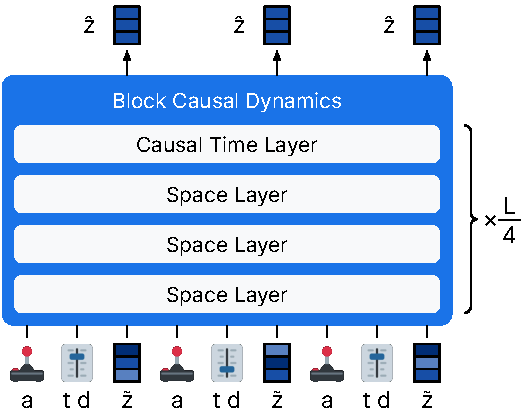
\includegraphics[height=2.5in]{figures/method/dyn}
\caption{Interactive Dynamics}
\end{subfigure}
\caption{World model design.
\method consists of a causal tokenizer and an interactive dynamics model, which both use the same block-causal transformer architecture.
The tokenizer encodes partially masked image patches and latent tokens, squeezes the latents through a low-dimensional projection with tanh activation, and decodes the patches.
It uses causal attention to achieve temporal compression while allowing frames to be decoded one by one.
The dynamics model operates on the interleaved sequence of actions, shortcut noise levels and step sizes, and tokenizer representations.
It denoises representations via a shortcut forcing objective.
After pretraining, the world model is finetuned into an agent by inserting task tokens into the dynamics transformer and predicting actions, rewards, and values from them.
}
\label{fig:model}
\end{figure}

\section{Previous Dreamer Generations}
\vspace*{-1ex}
Dreamer~3\citep{dreamerv3} learned to obtain diamonds in Minecraft from scratch by online interaction.
Its inputs are low-resolution images and inventory states and the outputs are mouse, keyboard, and abstract crafting actions.
Dreamer~3 uses a recurrent state-space model (RSSM) \citep{hafner2018planet} as its world model, which is based on a recurrent neural network and a variational objective.
This approach results in a lightweight world model with highly efficient inference but is difficult to scale to diverse data distributions.
In contrast, \method learns to obtain diamonds in Minecraft purely from offline data.
Its inputs are only high-resolution images and the outputs are low-level mouse and keyboard actions.
\method uses a scalable world model based on an efficient transformer architecture and a shortcut forcing objective, allowing it to scale to diverse data distributions with many details.
While Dreamer~3 uses return normalization and an entropy regularizer, \method uses PMPO with a KL to the behavioral cloning prior for imagination training, where no normalization is needed.
\vspace*{1ex}
\begin{figure}[t!]
\vspace*{-2\baselineskip}
\centering
\begin{subfigure}[t]{0.45\textwidth}
\centering
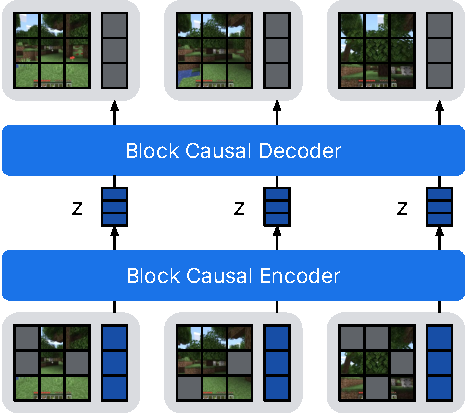
\includegraphics[height=2.4in]{figures/method/tok}
\caption{Causal Tokenizer}
\end{subfigure}%
\hfill%
\begin{subfigure}[t]{0.45\textwidth}
\centering
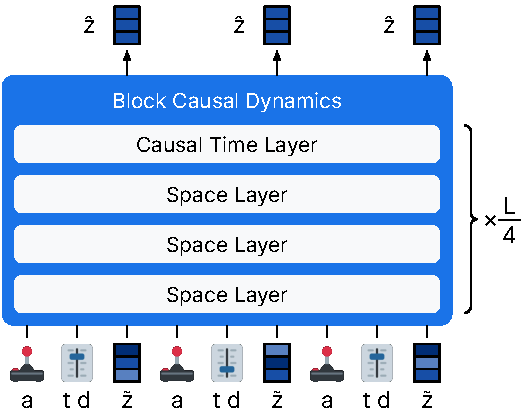
\includegraphics[height=2.5in]{figures/method/dyn}
\caption{Interactive Dynamics}
\end{subfigure}
\caption{World model design.
\method consists of a causal tokenizer and an interactive dynamics model, which both use the same block-causal transformer architecture.
The tokenizer encodes partially masked image patches and latent tokens, squeezes the latents through a low-dimensional projection with tanh activation, and decodes the patches.
It uses causal attention to achieve temporal compression while allowing frames to be decoded one by one.
The dynamics model operates on the interleaved sequence of actions, shortcut noise levels and step sizes, and tokenizer representations.
It denoises representations via a shortcut forcing objective.
After pretraining, the world model is finetuned into an agent by inserting task tokens into the dynamics transformer and predicting actions, rewards, and values from them.
}
\label{fig:model}
\end{figure}
\clearpage

\enlargethispage{\baselineskip}
\vspace*{-10ex}
\section{Human Interaction: Lucid-v1}
\vspace*{-2ex}
\begin{figure}[h!]
% \centering
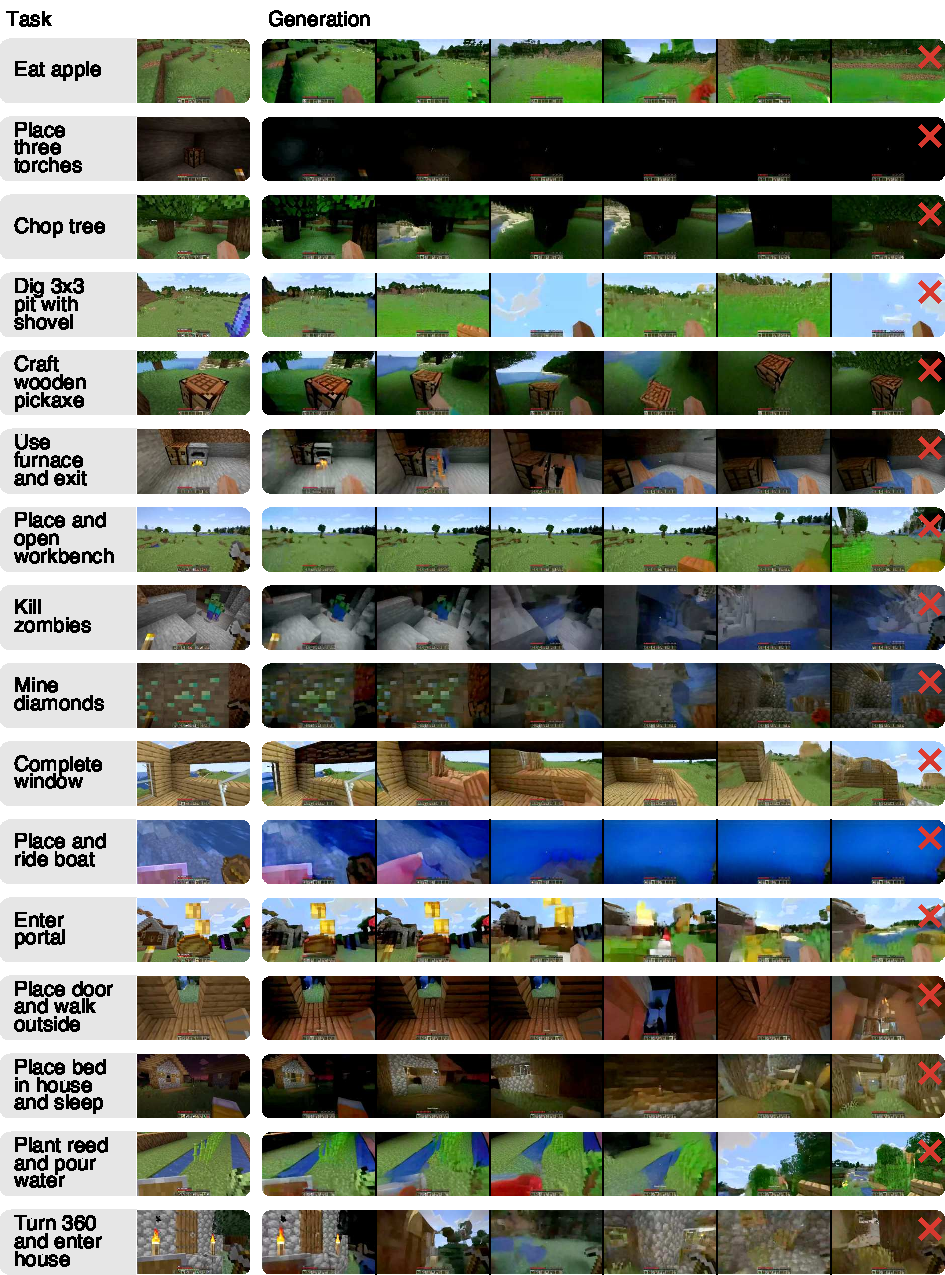
\includegraphics[width=0.97\linewidth]{figures/wmtasks/lucid}
\caption{Lucid-v1}
\label{fig:wmtasks_lucid}
\end{figure}
\vspace*{-2ex}
\clearpage

\enlargethispage{\baselineskip}
\vspace*{-10ex}
\section{Human Interaction: OASIS (large)}
\vspace*{-2ex}
\begin{figure}[h!]
% \centering
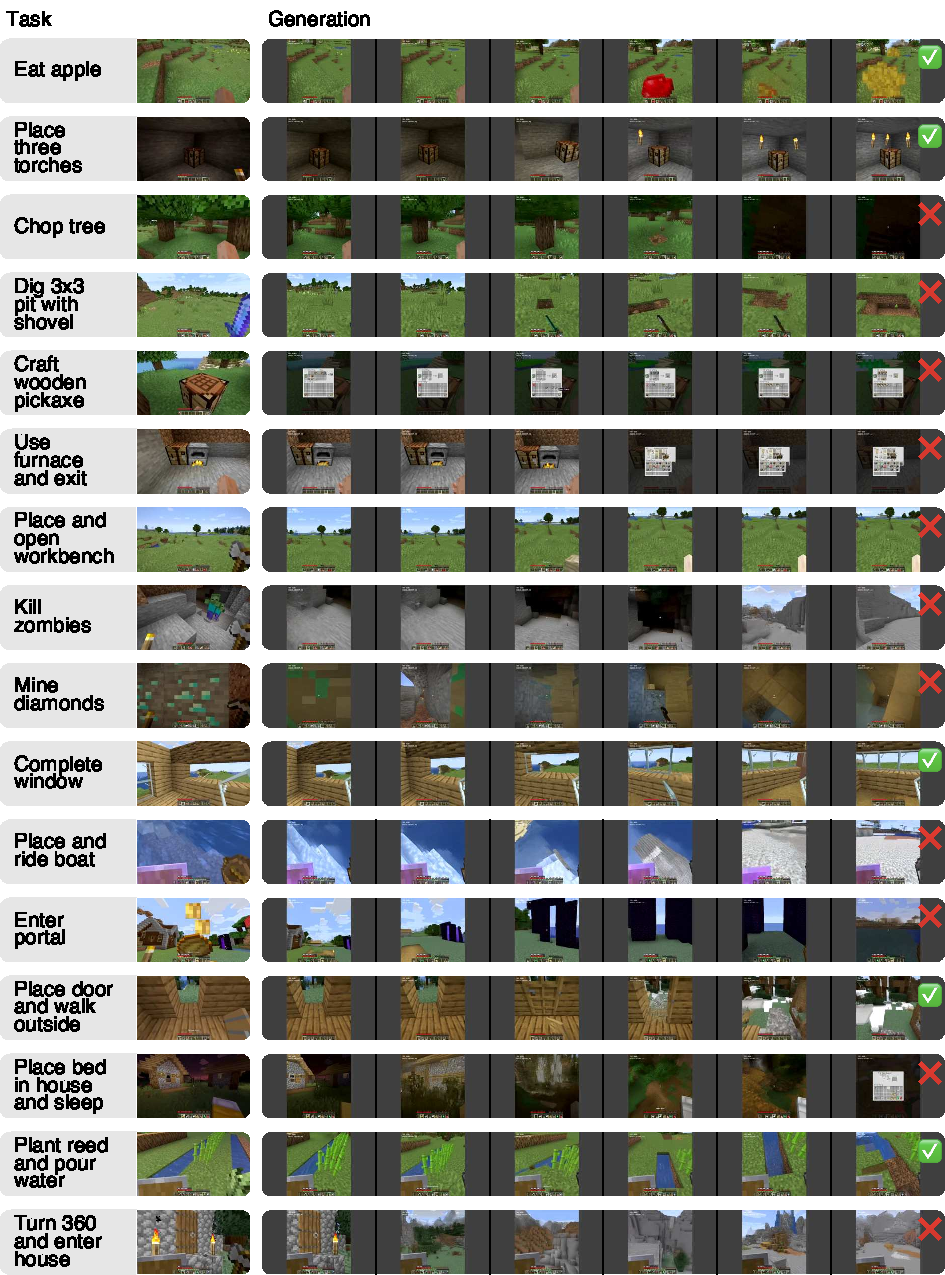
\includegraphics[width=0.97\linewidth]{figures/wmtasks/oasis}
\caption{Oasis (large)}
\label{fig:wmtasks_oasis}
\end{figure}
\vspace*{-2ex}
\clearpage

\enlargethispage{\baselineskip}
\vspace*{-10ex}
\section{Human Interaction: \method}
\vspace*{-2ex}
\begin{figure}[h!]
%\centering
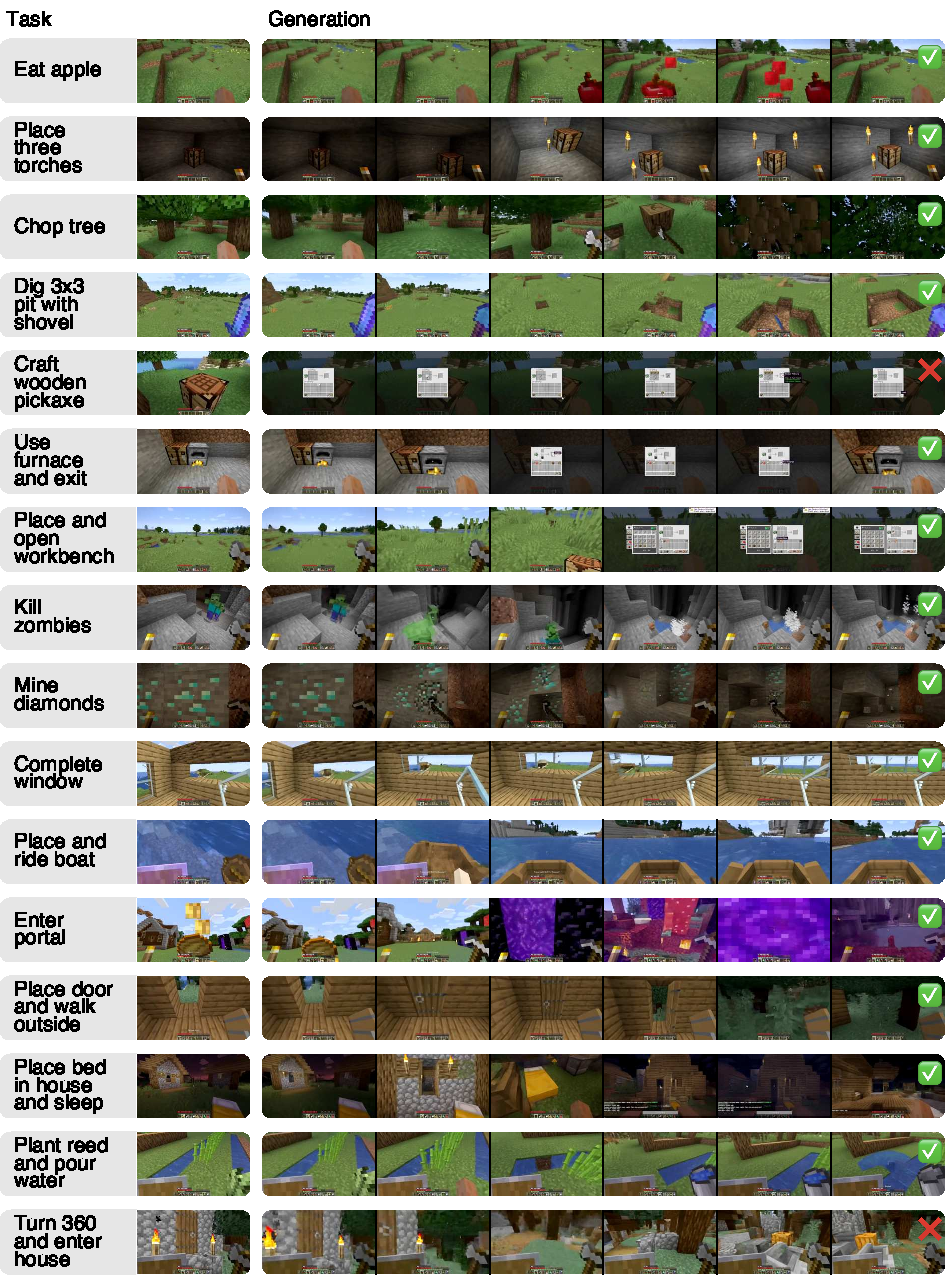
\includegraphics[width=0.97\linewidth]{figures/wmtasks/dreamer}
\caption{\method}
\label{fig:wmtasks_ours}
\end{figure}
\clearpage


\end{document}
